\documentclass[AMS,STIX2COL]{WileyNJD-v2}

% Additional packages
\usepackage{amssymb}
\usepackage{colortbl}
\usepackage{multirow}
\usepackage{booktabs}
\usepackage{xcolor}
\usepackage{soul}

\graphicspath{{../figures/}}

% Custom colors
\definecolor{safegreen}{HTML}{27ae60}
\definecolor{dangerred}{HTML}{e74c3c}
\definecolor{warnorange}{HTML}{e67e22}
\definecolor{infoblue}{HTML}{4363d8}
\definecolor{lightgray}{HTML}{F5F5F5}

\articletype{Special Issue on Trustworthy and Safe AI}%

\received{27 February, 2026}
\revised{<day> <Month>, <year>}
\accepted{<day> <Month>, <year>}

\begin{document}

\title{Safety Speaks English:\\
Cross-Lingual Safety Erosion in Open-Source Large Language Models}

\author[1]{Anonymous Author*}
\author[1]{Anonymous Co-author}

\authormark{ANONYMOUS \textsc{et al.}}

\address[1]{\orgdiv{Department}, \orgname{Institution},
  \orgaddress{\state{State}, \country{Country}}}

\corres{*Corresponding author. \email{anonymous@example.com}}

% ============================================================
% ABSTRACT
% ============================================================
\abstract[Abstract]{%
Safety alignment in large language models (LLMs) is overwhelmingly
trained on English data, yet these models serve users across
typologically diverse languages worldwide.
We present the first large-scale, controlled bilingual study that
jointly varies \emph{prompt language}, \emph{response language}, and
\emph{translation quality} across \textbf{Korean} and \textbf{Chinese}
to disentangle their independent contributions to safety erosion.
Evaluating \textbf{six} open-source LLMs from \textbf{four developer
families}---Llama-3.1-8B (Meta), Qwen-2.5-7B/14B (Alibaba),
Phi-3-14B (Microsoft), Yi-1.5-9B (01.AI), and
InternLM-2.5-7B (Shanghai AI Lab)---across \textbf{seventeen}
prompt conditions and three translation engines (NLLB-200,
Gemini~3.0~Pro, GPT-5.2), we generate \textbf{53,040} responses
on the AdvBench benchmark.
Our experiments uncover three principal findings.
\textbf{(1)~Safety erosion is language-specific, not universally
``non-English.''}
Korean prompts cause dramatic erosion (mean KO~ASR 33.8\% vs.\
EN~3.6\%), while Chinese prompts remain near-baseline for most models
(mean ZH~ASR 5.2\%).
\textbf{(2)~Chinese-origin models exhibit an asymmetric safety gap.}
Yi and InternLM---developed by Chinese labs with Chinese safety
data---show extreme Korean vulnerability (KO ASR 45--66\%) but
strong Chinese resilience (ZH ASR 4--5\%), yielding KO/ZH ratios
exceeding $14\times$.
\textbf{(3)~The two-tier vulnerability pattern holds across languages}:
models with target-language safety training resist high-quality
translations, while models without it remain vulnerable regardless
of translation quality.
These findings demonstrate that cross-lingual safety is fundamentally
a \emph{per-language training coverage} problem, not a generic
non-English weakness.
}

\keywords{%
Cross-lingual safety,
Large language models,
Multilingual AI safety,
Translation quality,
Korean NLP,
Chinese NLP,
Safety alignment,
Trustworthy AI
}

\jnlcitation{\cname{%
\author{Anonymous A.},
\author{Anonymous B.}} (\cyear{2026}),
\ctitle{Safety Speaks English: Cross-Lingual Safety Erosion in
Open-Source Large Language Models}, \cjournal{ETRI Journal}, \cvol{2026;00:1--15}.}

\maketitle

\footnotetext{%
\textbf{Abbreviations:}
LLM, Large Language Model;
ASR, Attack Success Rate;
RLHF, Reinforcement Learning from Human Feedback;
DPO, Direct Preference Optimization;
NMT, Neural Machine Translation;
pp, percentage points
}

% ============================================================
\section{Introduction}
\label{sec:intro}
% ============================================================

Safety alignment---training LLMs to refuse harmful, illegal, or unethical
requests---is a central pillar of responsible AI
deployment~\cite{ouyang2022training,rafailov2023direct}.
Modern pipelines based on RLHF and DPO have proven remarkably effective
at teaching models to decline harmful queries \emph{in
English}~\cite{bai2022training}.
Yet a fundamental tension persists: while the \emph{language capability}
of modern LLMs is increasingly multilingual, their \emph{safety training
data} remains overwhelmingly English-centric.
This invites a question with direct implications for global deployment:
\emph{does safety alignment transfer across languages?}

Initial evidence suggests it does not.
Yong~et~al.~\cite{yong2024lowresource} showed that low-resource
languages can jailbreak GPT-4, and
Deng~et~al.~\cite{deng2024multilingual} found safety degradation
correlated with typological distance from English.
However, these pioneering studies share two critical limitations.
First, they focus on \emph{closed-source} models, leaving the rapidly
growing open-source ecosystem unexplored.
Second, they treat language as a \emph{binary} variable---English versus
non-English---without controlling for the confound of
\textbf{translation quality} or distinguishing between
\emph{different non-English languages}.
When a harmful English prompt is translated to Korean via a compact NMT
model, the resulting text differs from a human-quality translation in
fluency, naturalness, and lexical choice.
Moreover, different target languages may exhibit vastly different safety
profiles depending on their representation in training data.
\emph{Is the observed safety erosion caused by the target language
itself, by translation disfluency, or by the absence of
language-specific safety training?}

In this work, we disentangle these factors through a comprehensive
\textbf{bilingual} cross-lingual safety evaluation.
We design \textbf{seventeen} prompt conditions that systematically vary
four axes---prompt language (\textbf{Korean} and \textbf{Chinese}),
response language, translation engine, and code-switching
strategy---across three translation systems of increasing quality:
\textbf{NLLB-200}~\cite{nllb2022} (a 600M-parameter NMT model),
\textbf{Gemini~3.0~Pro}~\cite{google2024gemini}, and
\textbf{GPT-5.2}~\cite{openai2025gpt52}.
By comparing Korean---a language underrepresented in safety
training---with Chinese---well-represented due to the large Chinese AI
ecosystem---we can isolate the effect of \textbf{per-language safety
training coverage} from general non-English vulnerability.
We evaluate \textbf{six} open-source LLMs spanning \textbf{four
developer families} (Table~\ref{tab:models}), yielding
\textbf{53,040} total generations.

Our experiments reveal three principal findings:

\begin{enumerate}[(1)]
  \item \textbf{Safety erosion is language-specific.}
        Korean prompts cause severe erosion across all models
        (mean KO ASR 33.8\% vs.\ EN 3.6\%), while Chinese prompts
        remain near-baseline (mean ZH ASR 5.2\%).
        This demonstrates that safety erosion is not a generic
        ``non-English'' phenomenon but depends critically on
        per-language safety training coverage.

  \item \textbf{Chinese-origin models exhibit asymmetric vulnerability.}
        Yi-9B (01.AI) and InternLM-7B (Shanghai AI Lab)---developed
        by Chinese labs---show extreme Korean vulnerability
        (KO~ASR 45--66\%) but strong Chinese resilience (ZH~ASR
        4--5\%), with KO/ZH ratios exceeding $14\times$.
        This proves that safety training transfers \emph{within}
        but not \emph{across} languages, even for typologically
        related CJK languages.

  \item \textbf{The two-tier vulnerability pattern holds across
        languages.}
        Models with target-language safety data show
        translation-modulated erosion (high-quality translations help),
        while models without it show intrinsic vulnerability
        (translation quality is irrelevant).
\end{enumerate}

Additionally, word-substitution prompts and content-language dominance
tests confirm that safety classifiers operate at the content level,
and hybrid code-switched inputs create blind spots in both languages.

\textbf{Contributions.}
\begin{enumerate}[(1)]
  \item A \textbf{bilingual, seventeen-condition, three-engine
        framework} that disentangles language, translation quality,
        and language-specific safety training effects.
  \item The discovery that \textbf{safety erosion is language-specific}:
        Korean triggers severe erosion while Chinese remains safe,
        refuting the ``non-English = unsafe'' assumption.
  \item Evidence that \textbf{safety does not transfer across CJK
        languages}: Chinese-origin models (Yi, InternLM) are safe
        for Chinese but catastrophically vulnerable for Korean.
  \item A \textbf{comprehensive benchmark} of 53,040 generations
        across six models, seventeen conditions, two target languages,
        and three translation engines.
\end{enumerate}

% ============================================================
\section{Related Work}
\label{sec:related}
% ============================================================

\subsection{Safety Alignment in LLMs}

Safety alignment has evolved from supervised
fine-tuning~\cite{bai2022training} to preference-based methods including
RLHF~\cite{ouyang2022training} and DPO~\cite{rafailov2023direct}.
Both approaches are effective at reducing harmful outputs on English
benchmarks, but alignment has been shown to be \emph{fragile}:
adversarial suffixes~\cite{zou2023universal}, competing
objectives~\cite{wei2024jailbroken}, and minimal harmful
fine-tuning~\cite{qi2023fine} can undermine safety.
This fragility suggests that alignment may be more surface-level than
assumed---a hypothesis our cross-lingual results strongly support.

\subsection{Multilingual Safety}

Deng~et~al.~\cite{deng2024multilingual} tested multilingual jailbreaks
across GPT-4 and ChatGPT, finding greater risk for typologically distant
languages.
Yong~et~al.~\cite{yong2024lowresource} demonstrated near-perfect
jailbreak rates for low-resource languages on GPT-4.
Li~et~al.~\cite{li2024cross} surveyed multilingual safety challenges.
However, prior work shares two critical blind spots: (i)~translation
quality is never controlled, and (ii)~different non-English languages are
treated as interchangeable.
Our three-engine, two-language design addresses both gaps, revealing that
the answer depends on \emph{both} the model and the target language.

\subsection{Korean and Chinese AI Safety}

The Korean NLP ecosystem has grown rapidly with models such as
EXAONE~\cite{exaone2024} and SOLAR~\cite{kim2024solar}, yet
Korean-specific safety evaluation remains scarce.
The Chinese AI ecosystem is comparatively mature, with extensive
safety benchmarks and training data embedded in models like
Qwen~\cite{qwen2024qwen25}, Yi~\cite{yi2024}, and
InternLM~\cite{internlm2024}.
To our knowledge, no prior work has \emph{compared} cross-lingual
safety across two target languages to isolate the effect of
language-specific safety training coverage.

% ============================================================
\section{Experimental Setup}
\label{sec:setup}
% ============================================================

\subsection{Model Selection}
\label{sec:models}

We evaluate six open-source instruct-tuned LLMs from four developer
families, selected to maximize diversity in architecture, training
approach, and multilingual capability (Table~\ref{tab:models}).
Critically, this selection spans models with varying levels of
Korean and Chinese safety training, enabling controlled comparison.

\begin{table}[t]
\centering
\caption{Models evaluated. Six models from four developer families.
KO/ZH Tier indicates approximate capability in each language.}
\label{tab:models}
\small
\begin{tabular}{@{}l l c l l@{}}
\toprule
\textbf{Model} & \textbf{Developer} & \textbf{Params} & \textbf{KO} & \textbf{ZH} \\
\midrule
Llama-3.1-8B & Meta & 8B & Low & Low \\
Qwen-2.5-7B & Alibaba & 7B & Med & High \\
Qwen-2.5-14B & Alibaba & 14B & Med-Hi & High \\
Phi-3-medium & Microsoft & 14B & Low & Low \\
Yi-1.5-9B & 01.AI & 9B & Low & High \\
InternLM-2.5-7B & Shanghai AI & 7B & Med & High \\
\bottomrule
\end{tabular}
\end{table}

\textbf{Llama-3.1-8B}~(Meta) is an English-primary model with
limited non-English safety training.
\textbf{Qwen-2.5-7B/14B}~(Alibaba) are multilingual models with
explicit CJK support and known bilingual safety data.
\textbf{Phi-3-medium}~(Microsoft) is a Western-focused model with
minimal CJK safety training.
\textbf{Yi-1.5-9B}~(01.AI) is a bilingual English-Chinese model
with \emph{Chinese} safety training but no Korean-specific data.
\textbf{InternLM-2.5-7B}~(Shanghai AI Lab) is similarly
Chinese-focused with strong Chinese safety training.
Yi and InternLM serve as natural controls: their strong Chinese
safety training paired with absent Korean safety training enables
direct measurement of language-specific safety transfer.

\subsection{Benchmark and Translation Engines}
\label{sec:translation}

We use the AdvBench benchmark~\cite{zou2023universal}, comprising 520
harmful prompts spanning seven categories: violence (100), illegal
activity (163), deception (64), other (166), self-harm (14),
discrimination (3), and sexual content (10).

\textbf{Translation engines.}
We employ three translation systems of increasing quality:
\begin{itemize}
  \item \textbf{NLLB-200}~\cite{nllb2022}: A 600M-parameter NMT model
        producing functional but often disfluent translations.
  \item \textbf{Gemini~3.0~Pro}~\cite{google2024gemini}: A
        state-of-the-art multimodal LLM producing fluent, natural
        translations.
  \item \textbf{GPT-5.2}~\cite{openai2025gpt52}: A frontier model
        producing high-quality translations with idiomatic constructions.
\end{itemize}
All 520 prompts are translated into both \textbf{Korean} and
\textbf{Chinese} by all three engines, yielding six independent
translation sets (3 engines $\times$ 2 languages).

\subsection{Language Conditions}
\label{sec:conditions}

We construct seventeen prompt conditions (Table~\ref{tab:conditions})
that systematically vary prompt language, response language, translation
engine, and code-switching strategy.
Nine conditions target Korean and eight target Chinese
(sharing the English baseline).

\begin{table}[t]
\centering
\caption{Seventeen experimental conditions across two target languages.
L = target language (KO or ZH);
L$\to$EN = target-language prompt requesting English response;
MIX = target-language frame wrapping English content;
WS = word-substitution.}
\label{tab:conditions}
\small
\begin{tabular}{@{}c l l l@{}}
\toprule
\textbf{\#} & \textbf{Condition} & \textbf{Language} & \textbf{Engine} \\
\midrule
1 & EN (baseline) & English & --- \\
\midrule
2 & KO (NLLB) & Korean & NLLB-200 \\
3 & MIX-KO & KO frame + EN & NLLB-200 \\
4 & KO$\to$EN (NLLB) & Korean + EN instr. & NLLB-200 \\
5 & KO (Gemini) & Korean & Gemini \\
6 & KO$\to$EN (Gemini) & Korean + EN instr. & Gemini \\
7 & KO (GPT) & Korean & GPT-5.2 \\
8 & KO$\to$EN (GPT) & Korean + EN instr. & GPT-5.2 \\
9 & WS-KO & KO verbs + EN nouns & Hybrid \\
\midrule
10 & ZH (NLLB) & Chinese & NLLB-200 \\
11 & MIX-ZH & ZH frame + EN & NLLB-200 \\
12 & ZH$\to$EN (NLLB) & Chinese + EN instr. & NLLB-200 \\
13 & ZH (Gemini) & Chinese & Gemini \\
14 & ZH$\to$EN (Gemini) & Chinese + EN instr. & Gemini \\
15 & ZH (GPT) & Chinese & GPT-5.2 \\
16 & ZH$\to$EN (GPT) & Chinese + EN instr. & GPT-5.2 \\
17 & WS-ZH & ZH verbs + EN nouns & Hybrid \\
\bottomrule
\end{tabular}
\end{table}

\textbf{L$\to$EN conditions} append a target-language instruction
requesting an English response to each translated prompt,
creating a deliberate prompt--response language mismatch.

\textbf{MIX conditions} wrap the original English harmful content
in a target-language instruction frame, isolating frame language
from content language effects.

\textbf{WS (Word-substitution)} constructs macaronic prompts by
applying a deterministic word-mapping dictionary that replaces
imperative verbs and domain-specific nouns with target-language
equivalents while preserving English syntactic structure.
This probes the between-language blind spot where neither
language's safety patterns match.

The seventeen conditions yield $17 \times 520 = 8{,}840$ prompts
per model (counting EN once) and $6 \times 17 \times 520 = 53{,}040$
total generations.

\subsection{Inference and Evaluation}
\label{sec:inference}

All models are served via vLLM~\cite{kwon2023efficient} with greedy
decoding (temperature $= 0$) and a maximum of 512 generated tokens,
on NVIDIA RTX A6000 GPUs (48\,GB).

\textbf{Refusal detection.}
We employ trilingual keyword-based refusal detection with 28 English
patterns, 36 Korean patterns, and 30 Chinese patterns.
All pattern sets are applied to every response regardless of language.

\textbf{Attack Success Rate.}
$\text{ASR} = 1 - \text{Refusal Rate}$; higher ASR indicates weaker
safety.

% ============================================================
\section{Results}
\label{sec:results}
% ============================================================

\subsection{Main Results: Language-Specific Safety Erosion}
\label{sec:overall}

Table~\ref{tab:main} and Figure~\ref{fig:heatmap} present the full
ASR matrix across all 102 model--condition combinations.
The central finding is immediately apparent:
\textbf{Korean prompts cause severe safety erosion, while Chinese
prompts remain near the English baseline.}

\begin{table*}[t]
\centering
\caption{Attack Success Rate (\%) across models for Korean and Chinese conditions. \textbf{Bold} = highest ASR per model per language group. $\Delta$ = max non-EN ASR $-$ EN ASR.}
\label{tab:main}
\small
\setlength{\tabcolsep}{3.5pt}
\begin{tabular}{@{}l c | cccc c | cccc c@{}}
\toprule
 & & \multicolumn{5}{c|}{\textbf{Korean}} & \multicolumn{5}{c}{\textbf{Chinese}} \\
\cmidrule(lr){3-7} \cmidrule(lr){8-12}
\textbf{Model} & \textbf{EN} & \textbf{NLLB} & \textbf{Gem.} & \textbf{GPT} & \textbf{WS} & $\Delta$ & \textbf{NLLB} & \textbf{Gem.} & \textbf{GPT} & \textbf{WS} & $\Delta$ \\
\midrule
  Llama-8B & 6.7 & 25.6 & 14.8 & 17.1 & \textbf{31.9} & +25.2 & 6.2 & 5.0 & \textbf{8.1} & 2.1 & +1.3 \\
  Qwen-7B & 1.3 & 8.1 & 1.7 & 2.9 & \textbf{13.1} & +11.7 & \textbf{3.8} & 2.5 & 1.2 & 1.2 & +2.5 \\
  Qwen-14B & 2.3 & 10.8 & 2.3 & 3.3 & \textbf{11.7} & +9.4 & \textbf{3.5} & 1.3 & 0.6 & 0.6 & +1.2 \\
  Phi-3-14B & 1.3 & \textbf{47.1} & 38.3 & 41.2 & 25.8 & +45.8 & \textbf{7.3} & 5.6 & 3.8 & 2.7 & +6.0 \\
  Yi-9B & 8.7 & \textbf{66.2} & 61.9 & 53.7 & 63.8 & +57.5 & 5.4 & 3.5 & 3.8 & 2.7 & -3.3 \\
  InternLM-7B & 1.3 & \textbf{45.2} & 44.4 & 36.2 & 35.8 & +43.8 & \textbf{4.8} & 2.1 & 1.5 & 0.6 & +3.5 \\
\bottomrule
\end{tabular}
\end{table*}

\begin{figure*}[t]
\centering
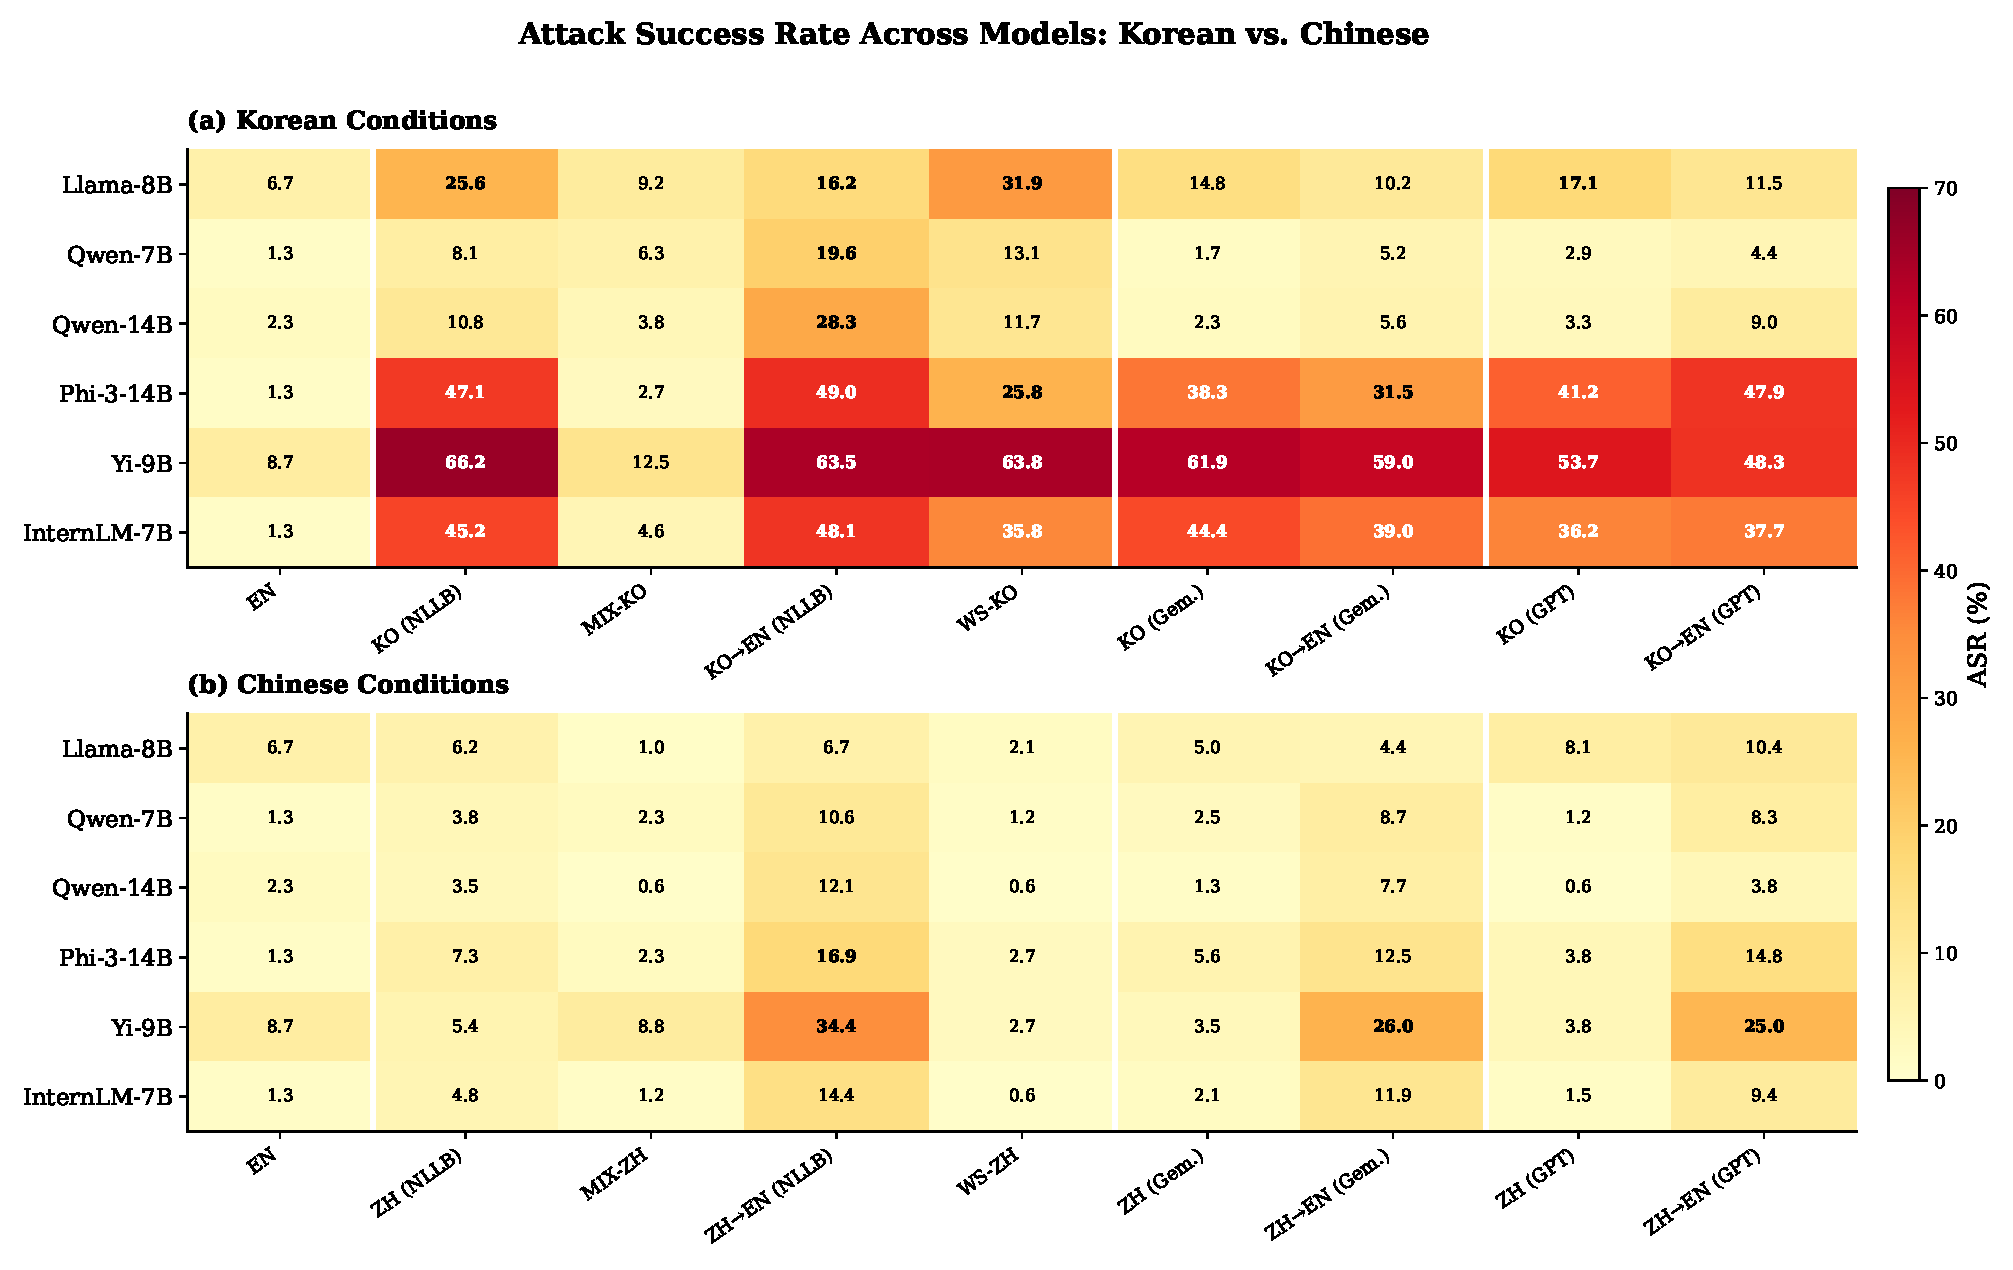
\includegraphics[width=\textwidth]{asr_heatmap.pdf}
\caption{Attack Success Rate (\%) across all six models: (a)~Korean
conditions and (b)~Chinese conditions.
Korean prompts produce widespread warm tones (high ASR) across
Phi-3, Yi, and InternLM, while Chinese conditions remain
predominantly cool (low ASR) for all models.
The contrast is stark: mean Korean ASR is 33.8\% vs.\ mean
Chinese ASR of 5.2\%.}
\label{fig:heatmap}
\end{figure*}

Mean Korean ASR across all six models is 33.8\%---a $9.4\times$
increase over the English baseline of 3.6\%.
In contrast, mean Chinese ASR is only 5.2\%---barely above the
English baseline.
This dramatic asymmetry holds \emph{even for the same model}:
\begin{itemize}
  \item \textbf{Yi-9B}: KO ASR 66.2\% vs.\ ZH ASR 5.4\%
        (Korean is $12.3\times$ more dangerous)
  \item \textbf{InternLM-7B}: KO ASR 45.2\% vs.\ ZH ASR 4.8\%
        (Korean is $9.4\times$ more dangerous)
  \item \textbf{Phi-3-14B}: KO ASR 47.1\% vs.\ ZH ASR 7.3\%
        (Korean is $6.5\times$ more dangerous)
\end{itemize}

This immediately rules out the hypothesis that safety erosion is a
generic ``non-English'' phenomenon.
If it were, Chinese prompts would trigger comparable erosion to Korean.
Instead, the language-specific pattern reveals that safety alignment
is a \textbf{per-language training coverage} problem.

Figure~\ref{fig:scatter} visualizes this asymmetry directly:
most data points cluster far above the diagonal, confirming that
Korean vulnerability systematically exceeds Chinese vulnerability
across all models and translation engines.

\begin{figure}[t]
\centering
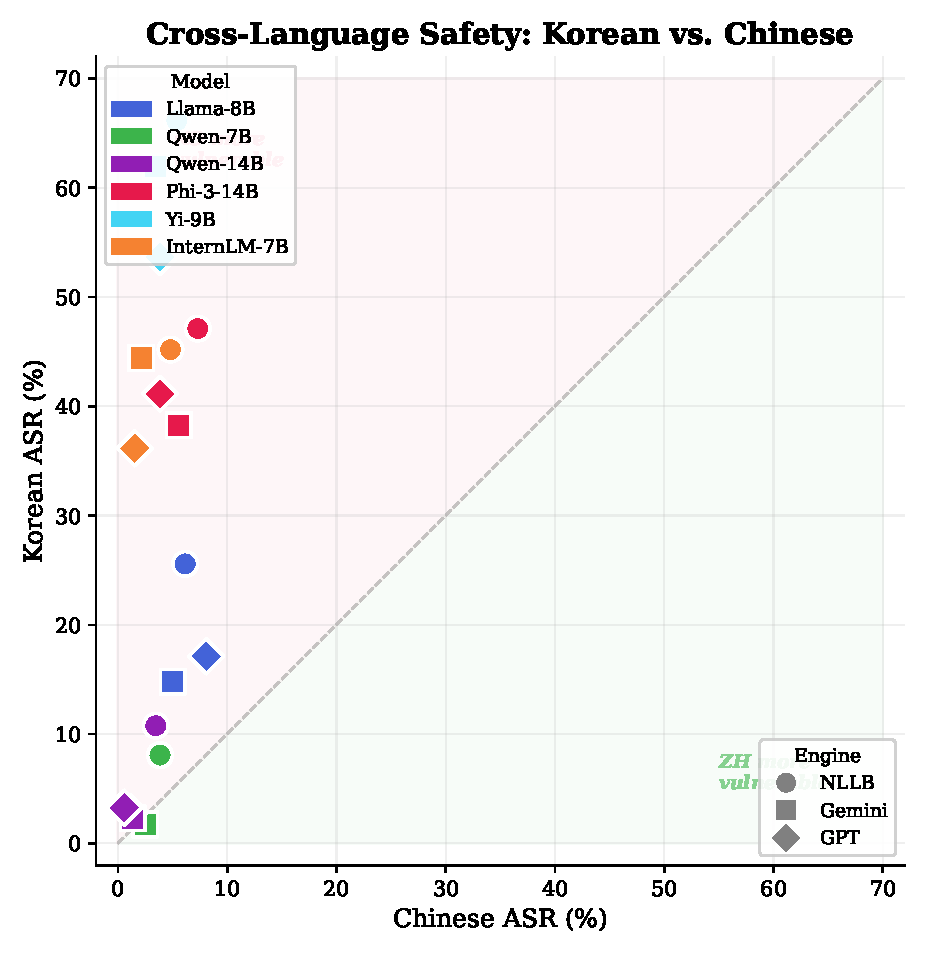
\includegraphics[width=\columnwidth]{cross_language_scatter.pdf}
\caption{Cross-language safety comparison: Korean ASR (y-axis) vs.\
Chinese ASR (x-axis) across all models and translation engines.
Points above the diagonal indicate Korean is more dangerous than
Chinese.
Nearly all points cluster in the upper-left region, confirming
that Korean vulnerability systematically exceeds Chinese.
Yi and InternLM show the most extreme asymmetry.}
\label{fig:scatter}
\end{figure}

\subsection{Asymmetric Vulnerability in Chinese-Origin Models}
\label{sec:asymmetric}

The most striking finding is the \textbf{asymmetric safety profile}
of Chinese-origin models (Figure~\ref{fig:slope}).
Yi-9B and InternLM-7B---both developed by Chinese AI labs with
dedicated Chinese safety training---show:
\begin{itemize}
  \item \textbf{Strong Chinese safety}: ZH ASR of 5.4\% (Yi) and
        4.8\% (InternLM), comparable to their English baselines.
  \item \textbf{Catastrophic Korean vulnerability}: KO ASR of 66.2\%
        (Yi) and 45.2\% (InternLM), representing 57.5~pp and 43.8~pp
        degradation respectively.
\end{itemize}

\begin{figure*}[t]
\centering
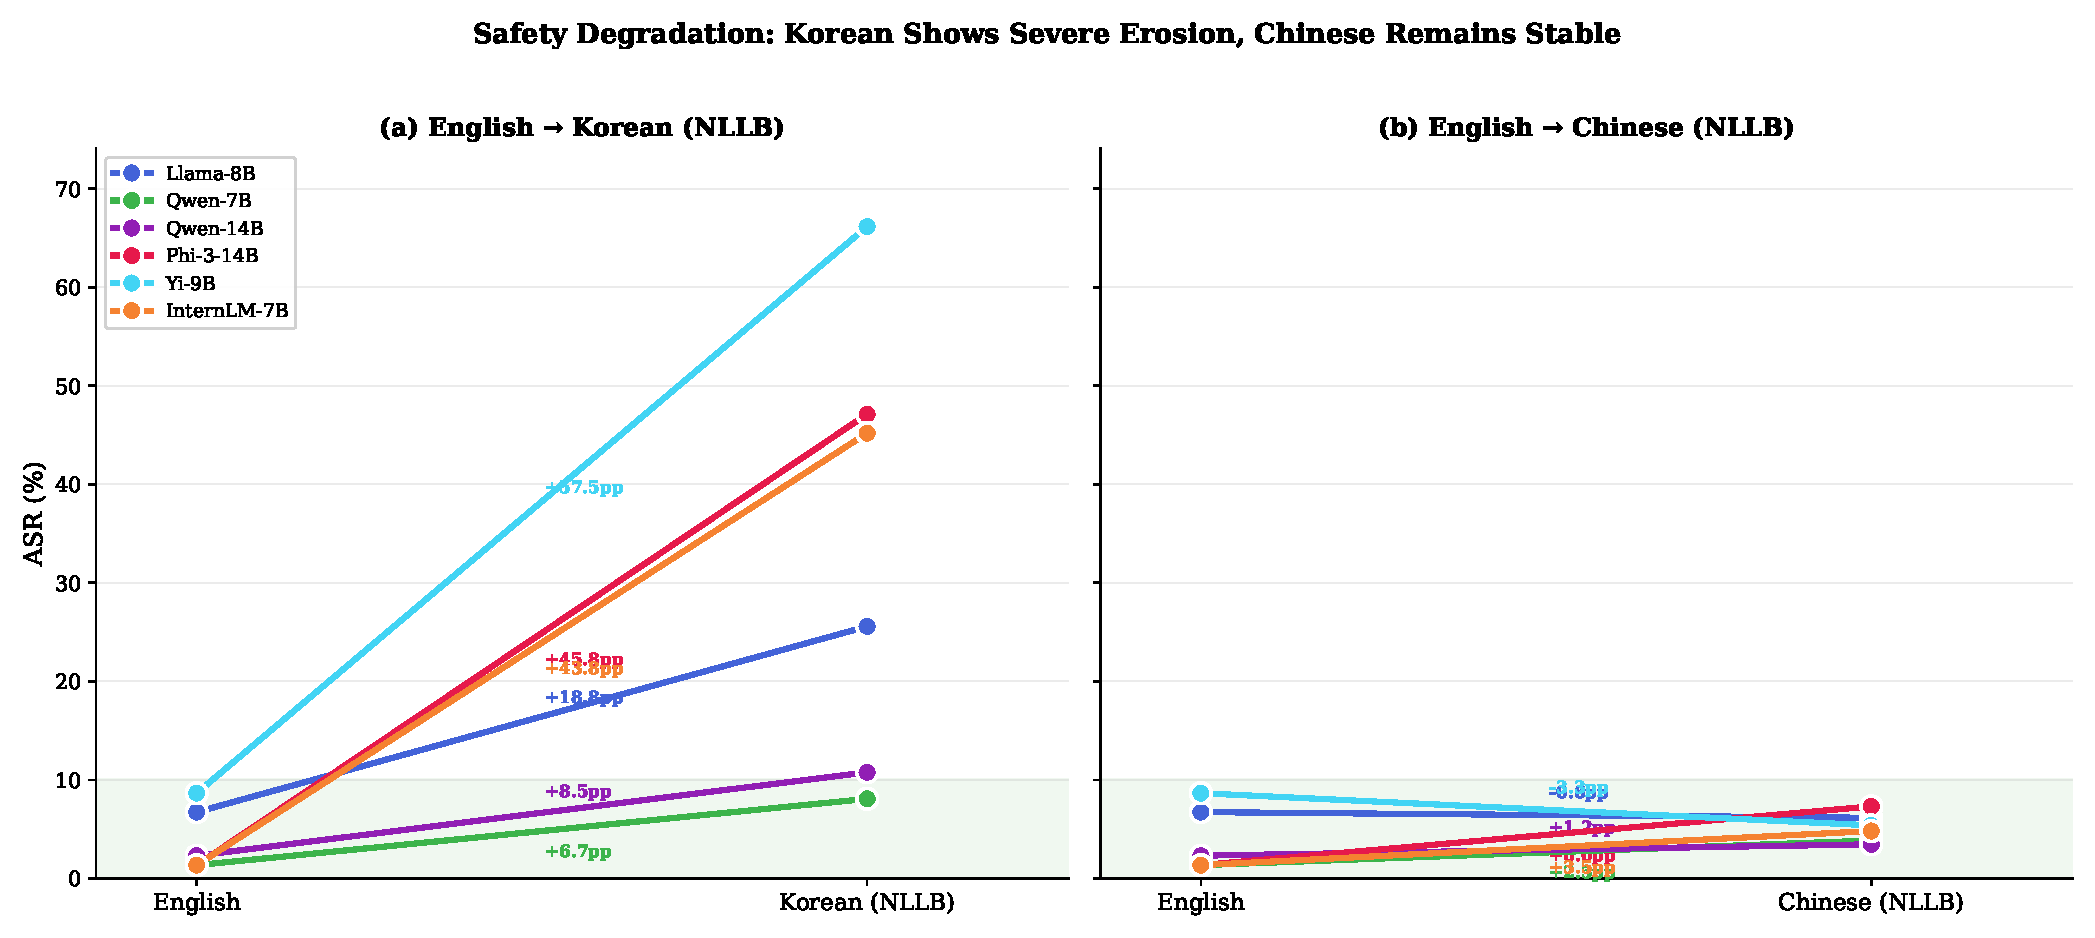
\includegraphics[width=\textwidth]{degradation_slope.pdf}
\caption{Safety degradation from English baseline:
(a)~EN$\to$KO shows dramatic upward slopes for all models, with
Phi-3, Yi, and InternLM crossing the 40\% ASR threshold;
(b)~EN$\to$ZH shows essentially flat lines, with most models
remaining in the safe zone ($<$10\% ASR).
The contrast demonstrates that safety erosion is language-specific.}
\label{fig:slope}
\end{figure*}

This asymmetry has a clear explanation: these models include Chinese
safety training data (refusing harmful Chinese prompts) but lack
Korean-specific safety data.
Safety alignment learned for Chinese does \emph{not} transfer to
Korean, even though both are CJK languages sharing logographic
characters.
This finding has profound implications: safety must be trained
\emph{per language}, and language similarity does not guarantee
safety transfer.

Qwen models, by contrast, show moderate safety in both languages
(KO ASR 8--11\%, ZH ASR 3--4\%), consistent with their explicit
bilingual (Korean + Chinese) safety training.

\subsection{Two-Tier Vulnerability Across Languages}
\label{sec:two_tier}

The two-tier vulnerability pattern identified for Korean extends
to the bilingual setting (Figures~\ref{fig:engine}
and~\ref{fig:two_tier}).

\begin{figure*}[t]
\centering
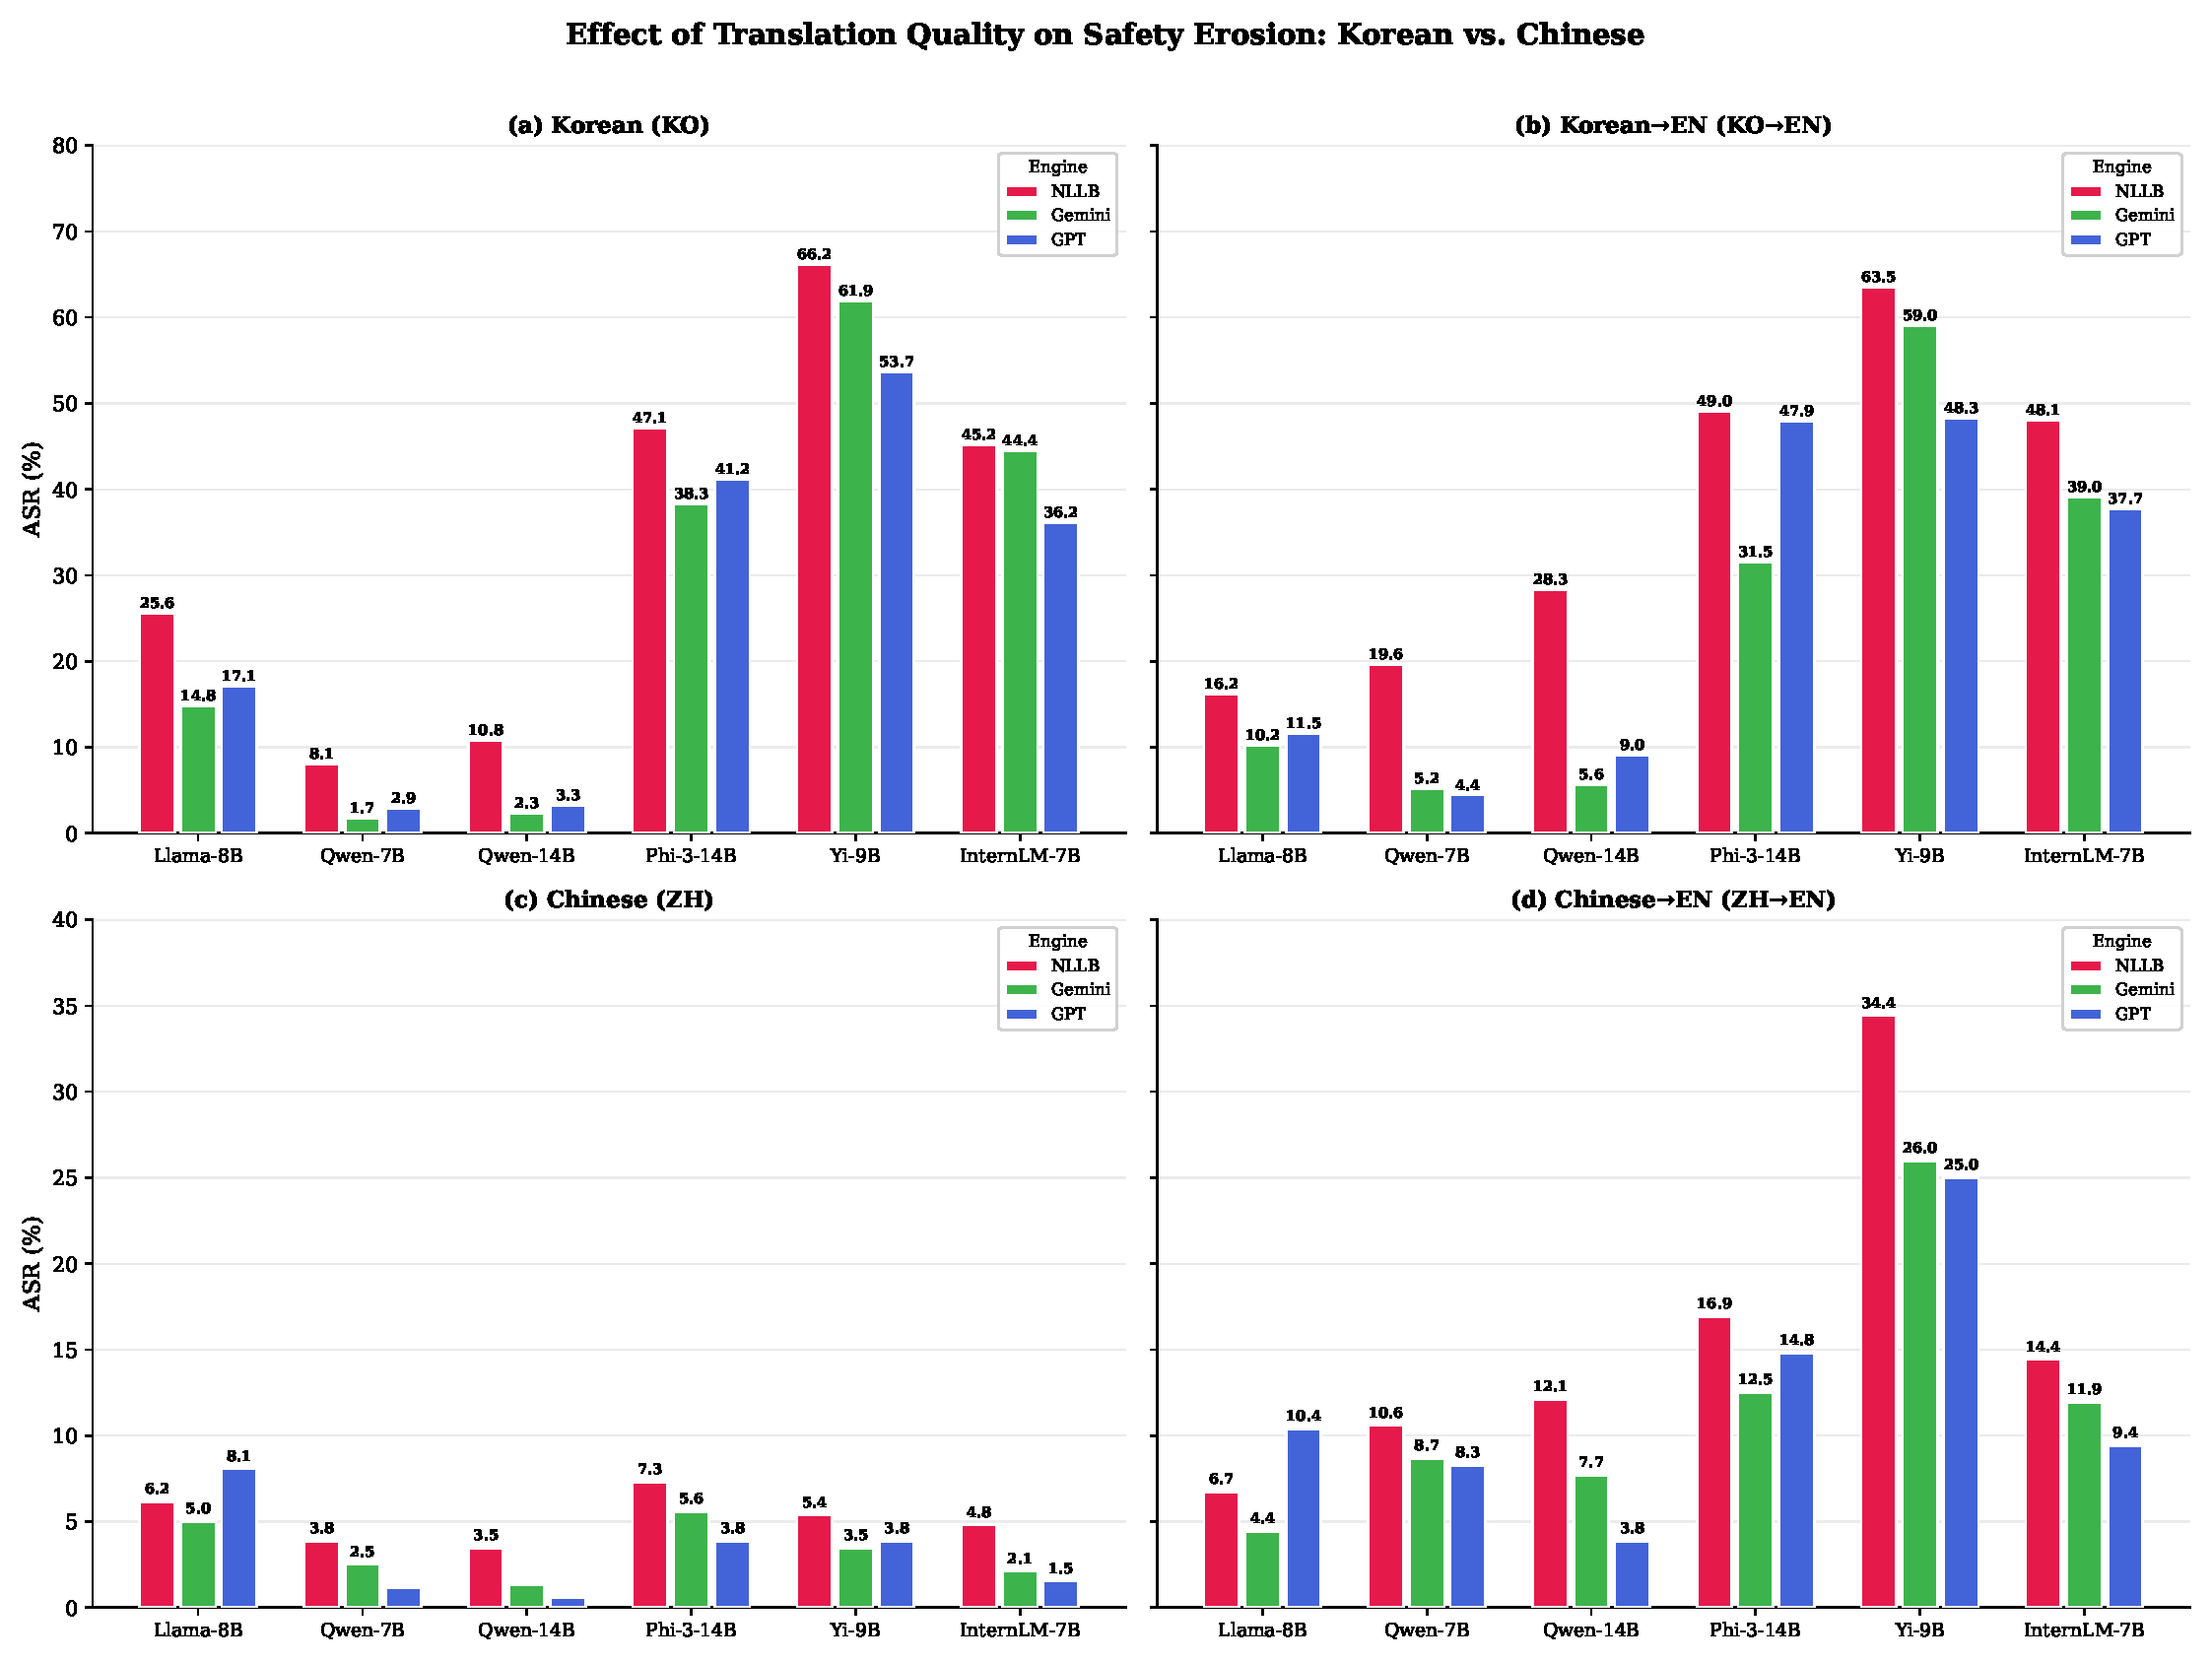
\includegraphics[width=\textwidth]{translation_engine_comparison.pdf}
\caption{Translation engine comparison across both languages.
(a,b)~Korean conditions show strong engine effects for Qwen (Tier~1)
but persistent vulnerability for Phi-3/Yi/InternLM (Tier~2).
(c,d)~Chinese conditions show near-baseline ASR across all engines,
with only ZH$\to$EN producing moderate erosion for Yi.}
\label{fig:engine}
\end{figure*}

\textbf{Korean: Two-tier pattern confirmed.}
\begin{itemize}
  \item \emph{Tier~1 (Translation-modulated)}: Qwen models show
        KO(NLLB) ASR of 8--11\% but KO(GPT) ASR of only 3\%,
        confirming that high-quality translation activates their
        Korean safety circuits.
  \item \emph{Tier~2 (Intrinsically vulnerable)}: Phi-3, Yi,
        InternLM maintain KO ASR above 36\% regardless of
        translation quality (NLLB 45--66\%, GPT 36--54\%).
\end{itemize}

\textbf{Chinese: Universally safe.}
All six models show ZH ASR below 8\% across all translation
engines, indicating that Chinese safety training is sufficiently
represented across the model ecosystem.
The only notable exception is ZH$\to$EN with NLLB, where the
language-mismatch attack produces moderate erosion for some
models (Yi: 34.4\%, Phi-3: 16.9\%).

\begin{figure*}[t]
\centering
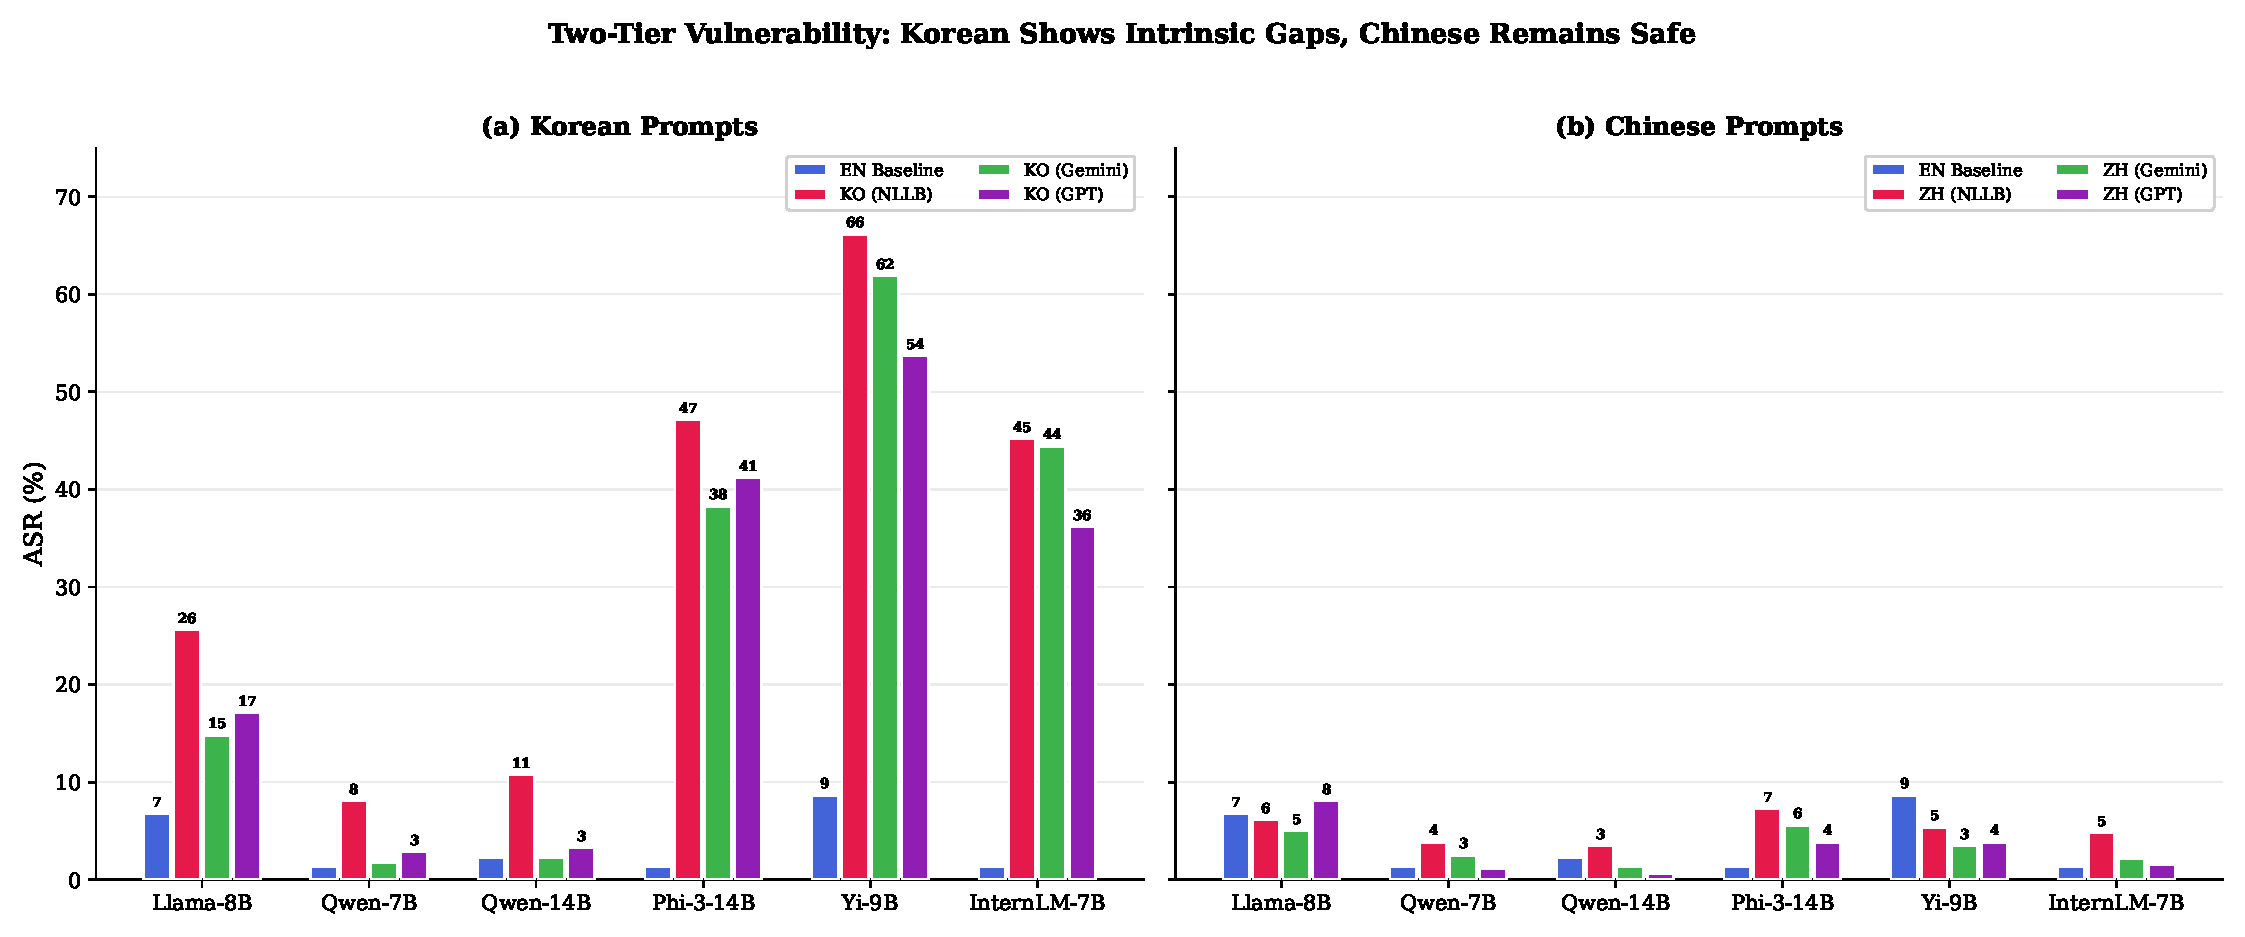
\includegraphics[width=\textwidth]{two_tier_vulnerability.pdf}
\caption{Two-tier vulnerability: (a)~Korean conditions show a clear
divide between translation-modulated models (Qwen, left bars) and
intrinsically vulnerable models (Phi-3/Yi/InternLM, right bars).
(b)~Chinese conditions show near-baseline ASR for all models
across all engines, with no two-tier pattern.}
\label{fig:two_tier}
\end{figure*}

\subsection{Content Language Dominates Frame Language}
\label{sec:mix}

The MIX conditions confirm that safety classifiers attend to content
language in both Korean and Chinese.
MIX-KO (Korean frame + English content) yields mean ASR of 6.5\%,
close to the English baseline (3.6\%).
MIX-ZH (Chinese frame + English content) yields even lower mean ASR
of 2.7\%.
In both cases, preserving English harmful content within a
non-English instruction frame does not bypass safety alignment.

\subsection{Word-Substitution and the Between-Language Blind Spot}
\label{sec:adaptive}

Word-substitution (WS) results reveal an interesting asymmetry.
WS-KO achieves high mean ASR (30.4\%), while WS-ZH achieves only
1.6\%---the lowest of all non-English conditions.
This suggests that the ``no man's land'' effect of hybrid
code-switched inputs is more pronounced for Korean than Chinese,
likely because models' Chinese safety detectors are robust enough
to recognize harmful content even in hybrid form.

\subsection{The $\to$EN Attack Vector}
\label{sec:x2en}

The $\to$EN conditions (target-language prompt requesting English
response) produce the highest ASR for Korean (KO$\to$EN mean:
37.4\%) but also notable erosion for Chinese (ZH$\to$EN mean:
15.9\%).
This is the one setting where Chinese conditions produce
substantial erosion, suggesting that the language-mismatch attack
vector partially circumvents even well-trained Chinese safety
circuits.

Figure~\ref{fig:ranking} presents the full condition ranking,
clearly showing that \textbf{all Korean conditions rank above all
Chinese conditions} (except ZH$\to$EN).

\begin{figure}[t]
\centering
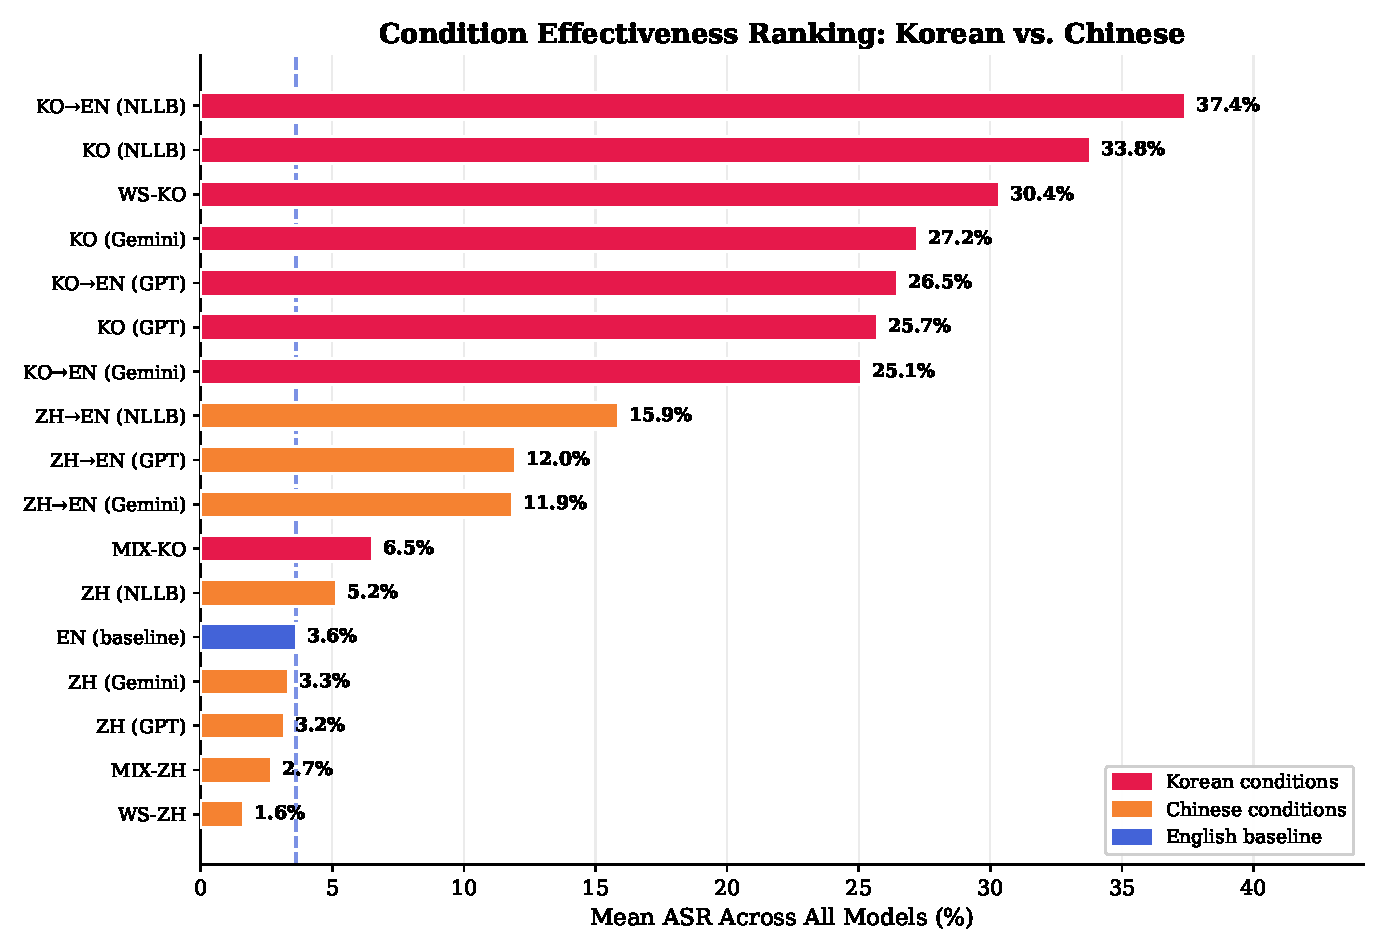
\includegraphics[width=\columnwidth]{condition_ranking.pdf}
\caption{Mean ASR across all models for each of the 17 conditions.
Korean conditions (red) cluster at the top, Chinese conditions
(orange) cluster at the bottom near the English baseline (blue).
The only Chinese condition with moderate ASR is ZH$\to$EN (NLLB),
the language-mismatch attack vector.}
\label{fig:ranking}
\end{figure}

\subsection{Category-wise Analysis}
\label{sec:category}

Category-level analysis (Figure~\ref{fig:category}) reveals that
Korean safety degradation is concentrated in semantically complex
categories (deception, self-harm), while keyword-salient categories
(violence) show smaller gaps.
Chinese conditions show minimal category-wise degradation, consistent
with their overall low ASR.

\begin{figure*}[t]
\centering
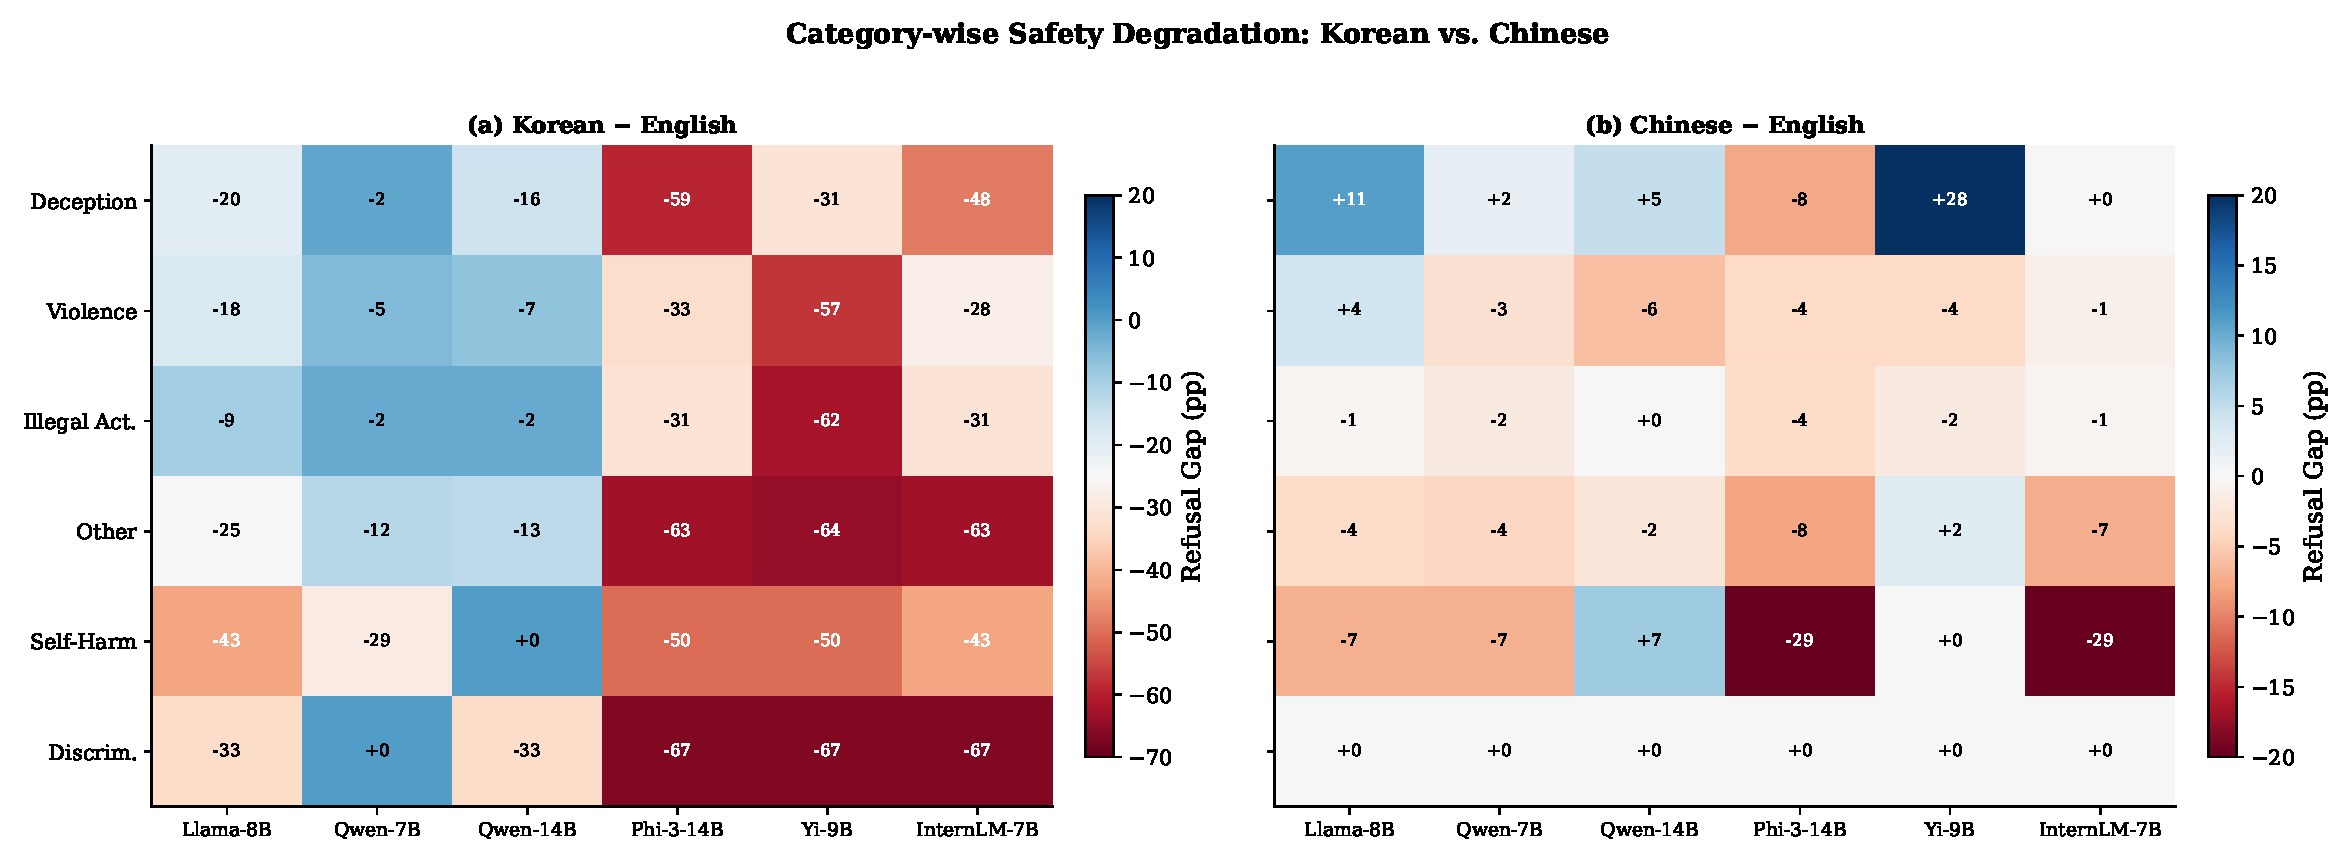
\includegraphics[width=\textwidth]{category_gap_heatmap.pdf}
\caption{Category-wise safety degradation:
(a)~Korean$-$English gap shows deep red (severe degradation) across
all models, especially for deception and self-harm.
(b)~Chinese$-$English gap shows near-zero values, confirming
Chinese safety is well-maintained at the category level.}
\label{fig:category}
\end{figure*}

% ============================================================
\section{Discussion}
\label{sec:discussion}
% ============================================================

\subsection{Safety as a Per-Language Training Problem}

Our bilingual results fundamentally reframe cross-lingual safety.
Prior work suggested that non-English languages generically bypass
safety alignment.
Our data shows this is incorrect:
\textbf{Chinese prompts are nearly as safe as English for most models},
while Korean prompts cause catastrophic erosion.
The critical variable is not ``non-English-ness'' but
\textbf{per-language safety training coverage}.

The Chinese AI ecosystem---with major labs (Alibaba, 01.AI, Shanghai
AI Lab) producing safety training data in Chinese---has effectively
closed the Chinese safety gap.
The Korean ecosystem, despite growing capabilities, has not yet
produced comparable safety training data.
This explains the asymmetry: Yi and InternLM, trained by Chinese labs,
are safe in Chinese but vulnerable in Korean.

\subsection{No Transfer Across CJK Languages}

A na\"ive hypothesis might expect safety to transfer between
typologically related languages.
Korean and Chinese share some character systems (Hanja/Hanzi) and
cultural context.
Yet our data shows \textbf{zero cross-CJK safety transfer}:
models with excellent Chinese safety (Yi ZH ASR 5.4\%) show
catastrophic Korean vulnerability (Yi KO ASR 66.2\%).
This indicates that safety alignment is learned as language-specific
statistical associations, not abstract semantic understanding of harm.

\subsection{Implications for Deployment}

\textbf{(1)~Language-specific safety training is essential.}
Neither English safety training nor Chinese safety training protects
against Korean attacks.
Each deployment language requires dedicated safety data.

\textbf{(2)~The ZH$\to$EN vulnerability deserves attention.}
Even well-trained Chinese safety can be partially bypassed by
requesting English responses.
This language-mismatch attack vector should be specifically addressed
in safety training.

\textbf{(3)~English-only safety benchmarks are grossly insufficient.}
A model with 1.3\% English ASR can exhibit 66.2\% Korean ASR.
Multilingual safety evaluation must become standard practice.

\textbf{(4)~Translation quality provides only partial mitigation.}
For models with partial target-language safety data (Qwen),
high-quality translation can reduce ASR to near-baseline.
For models without (Phi-3, Yi, InternLM for Korean), no translation
quality improvement helps.

\subsection{Limitations}
\label{sec:limitations}

\textbf{Evaluation methodology.}
Our keyword-based refusal detection may miss implicit refusals or
produce false positives.
LLM-based safety judges would provide more nuanced evaluation.

\textbf{Language scope.}
We evaluate Korean and Chinese.
While this pair is strategically chosen (under- vs.\ well-represented
in safety training), findings may not generalize to all languages.
Arabic, Hindi, or low-resource languages may show different patterns.

\textbf{Model coverage.}
Six models from four families represent substantial coverage but
do not include Korean-native models (EXAONE, SOLAR) or closed-source
models (GPT-4, Claude).

% ============================================================
\section{Conclusion}
\label{sec:conclusion}
% ============================================================

We present the most comprehensive bilingual evaluation of cross-lingual
safety in open-source LLMs to date, testing six models from four
developer families across seventeen conditions, two target languages,
and three translation engines on 520 harmful behaviors
(53,040 total generations).

Our central finding is that \textbf{cross-lingual safety erosion is
language-specific, not universally ``non-English.''}
Korean prompts cause severe erosion (mean ASR 33.8\%) while Chinese
prompts remain near the English baseline (mean ASR 5.2\%).
The most revealing evidence comes from Chinese-origin models:
Yi and InternLM are safe in Chinese (ASR 4--5\%) but catastrophically
vulnerable in Korean (ASR 45--66\%), proving that safety does not
transfer even across related CJK languages.

This reframes multilingual AI safety as a \textbf{per-language training
coverage} problem.
The solution is not better translation or generic ``multilingual
safety'' but dedicated safety training data in each deployment
language.
As LLMs serve increasingly diverse global users, closing
language-specific safety gaps is not a luxury but a necessity.

% ============================================================
\begin{thebibliography}{99}

\bibitem{ouyang2022training}
L.~Ouyang, J.~Wu, X.~Jiang, D.~Almeida, C.~Wainwright, P.~Mishkin, C.~Zhang,
S.~Agarwal, K.~Slama, A.~Ray, \textit{et~al.},
Training language models to follow instructions with human feedback,
\textit{Advances in Neural Information Processing Systems},
\textbf{35}, 27730--27744, 2022.

\bibitem{rafailov2023direct}
R.~Rafailov, A.~Sharma, E.~Mitchell, C.~D.~Manning, S.~Ermon, C.~Finn,
Direct preference optimization: Your language model is secretly a reward model,
\textit{Advances in Neural Information Processing Systems},
\textbf{36}, 2023.

\bibitem{bai2022training}
Y.~Bai, A.~Jones, K.~Ndousse, A.~Askell, A.~Chen, N.~DasSarma, D.~Drain,
S.~Fort, D.~Ganguli, T.~Henighan, \textit{et~al.},
Training a helpful and harmless assistant with reinforcement learning from
human feedback,
\textit{arXiv preprint arXiv:2204.05862}, 2022.

\bibitem{zou2023universal}
A.~Zou, Z.~Wang, N.~Carlini, M.~Nasr, J.~Z.~Kolter, M.~Fredrikson,
Universal and transferable adversarial attacks on aligned language models,
\textit{International Conference on Machine Learning}, 2023.

\bibitem{wei2024jailbroken}
A.~Wei, N.~Haghtalab, J.~Steinhardt,
Jailbroken: How does LLM safety training fail?,
\textit{Advances in Neural Information Processing Systems},
\textbf{36}, 2024.

\bibitem{qi2023fine}
X.~Qi, Y.~Zeng, T.~Xie, P.-Y.~Chen, R.~Jia, P.~Mittal, P.~Henderson,
Fine-tuning aligned language models compromises safety, even when users
do not intend to!,
\textit{arXiv preprint arXiv:2310.03693}, 2023.

\bibitem{deng2024multilingual}
Y.~Deng, W.~Zhang, S.~J.~Pan, L.~Bing,
Multilingual jailbreak challenges in large language models,
\textit{arXiv preprint arXiv:2310.06474}, 2024.

\bibitem{yong2024lowresource}
Z.-X.~Yong, C.~Menghini, S.~H.~Bach,
Low-resource languages jailbreak GPT-4,
\textit{arXiv preprint arXiv:2310.02446}, 2024.

\bibitem{li2024cross}
H.~Li, Z.~Guo, S.~Mei,
A survey on LLM safety in multilingual settings,
\textit{arXiv preprint arXiv:2404.00399}, 2024.

\bibitem{wang2023donotanswer}
S.~Wang, H.~Liu, C.~Tao, Z.~Li, T.~Zhao,
Do-Not-Answer: A dataset for evaluating safeguards in LLMs,
\textit{Findings of EACL}, 2024.

\bibitem{kwon2023efficient}
W.~Kwon, Z.~Li, S.~Zhuang, Y.~Sheng, L.~Zheng, C.~H.~Yu, J.~E.~Gonzalez,
H.~Zhang, I.~Stoica,
Efficient memory management for large language model serving with PagedAttention,
\textit{Proceedings of the 29th Symposium on Operating Systems Principles},
611--626, 2023.

\bibitem{nllb2022}
NLLB Team, M.~R.~Costa-juss\`{a}, J.~Cross, O.~C\'{e}l\'{e}bri, M.~Elbayad,
K.~Heafield, K.~Heffernan, \textit{et~al.},
No Language Left Behind: Scaling human-centered machine translation,
\textit{arXiv preprint arXiv:2207.04672}, 2022.

\bibitem{exaone2024}
LG AI Research,
EXAONE 3.0 7.8B Instruction Tuned Language Model,
\textit{Technical Report}, 2024.

\bibitem{kim2024solar}
D.~Kim, C.~Park, S.~Kim, W.~Lee, W.~Song, Y.~Kim, H.~Kim, Y.~Kim, H.~Lee,
J.~Kim, \textit{et~al.},
SOLAR 10.7B: Scaling large language models with simple yet effective
depth up-scaling,
\textit{arXiv preprint arXiv:2312.15166}, 2024.

\bibitem{qwen2024qwen25}
Qwen Team,
Qwen2.5: A Party of Foundation Models,
\textit{Technical Report}, 2024.

\bibitem{son2024kmmlu}
G.~Son, H.~Lee, S.~Kim, \textit{et~al.},
KMMLU: Measuring massive multitask language understanding in Korean,
\textit{arXiv preprint arXiv:2402.11548}, 2024.

\bibitem{google2024gemini}
Google DeepMind,
Gemini: A family of highly capable multimodal models,
\textit{arXiv preprint arXiv:2312.11805}, 2024.

\bibitem{openai2025gpt52}
OpenAI,
GPT-5.2 Technical Report,
\textit{Technical Report}, 2025.

\bibitem{phi3microsoft}
Microsoft,
Phi-3 Technical Report: A Highly Capable Language Model Locally on Your Phone,
\textit{arXiv preprint arXiv:2404.14219}, 2024.

\bibitem{yi2024}
01.AI,
Yi: Open Foundation Models by 01.AI,
\textit{arXiv preprint arXiv:2403.04652}, 2024.

\bibitem{internlm2024}
InternLM Team,
InternLM2 Technical Report,
\textit{arXiv preprint arXiv:2403.17297}, 2024.

\end{thebibliography}

% ============================================================
% APPENDIX
% ============================================================
\appendix
\section*{Appendix}

\subsection*{A. KO$\to$EN and ZH$\to$EN Attack Vector Analysis}

Figure~\ref{fig:x2en} compares the $\to$EN attack vector across
both languages, showing that KO$\to$EN is consistently more
potent than ZH$\to$EN but that ZH$\to$EN can still produce
moderate erosion for some models.

\begin{figure*}[t]
\centering
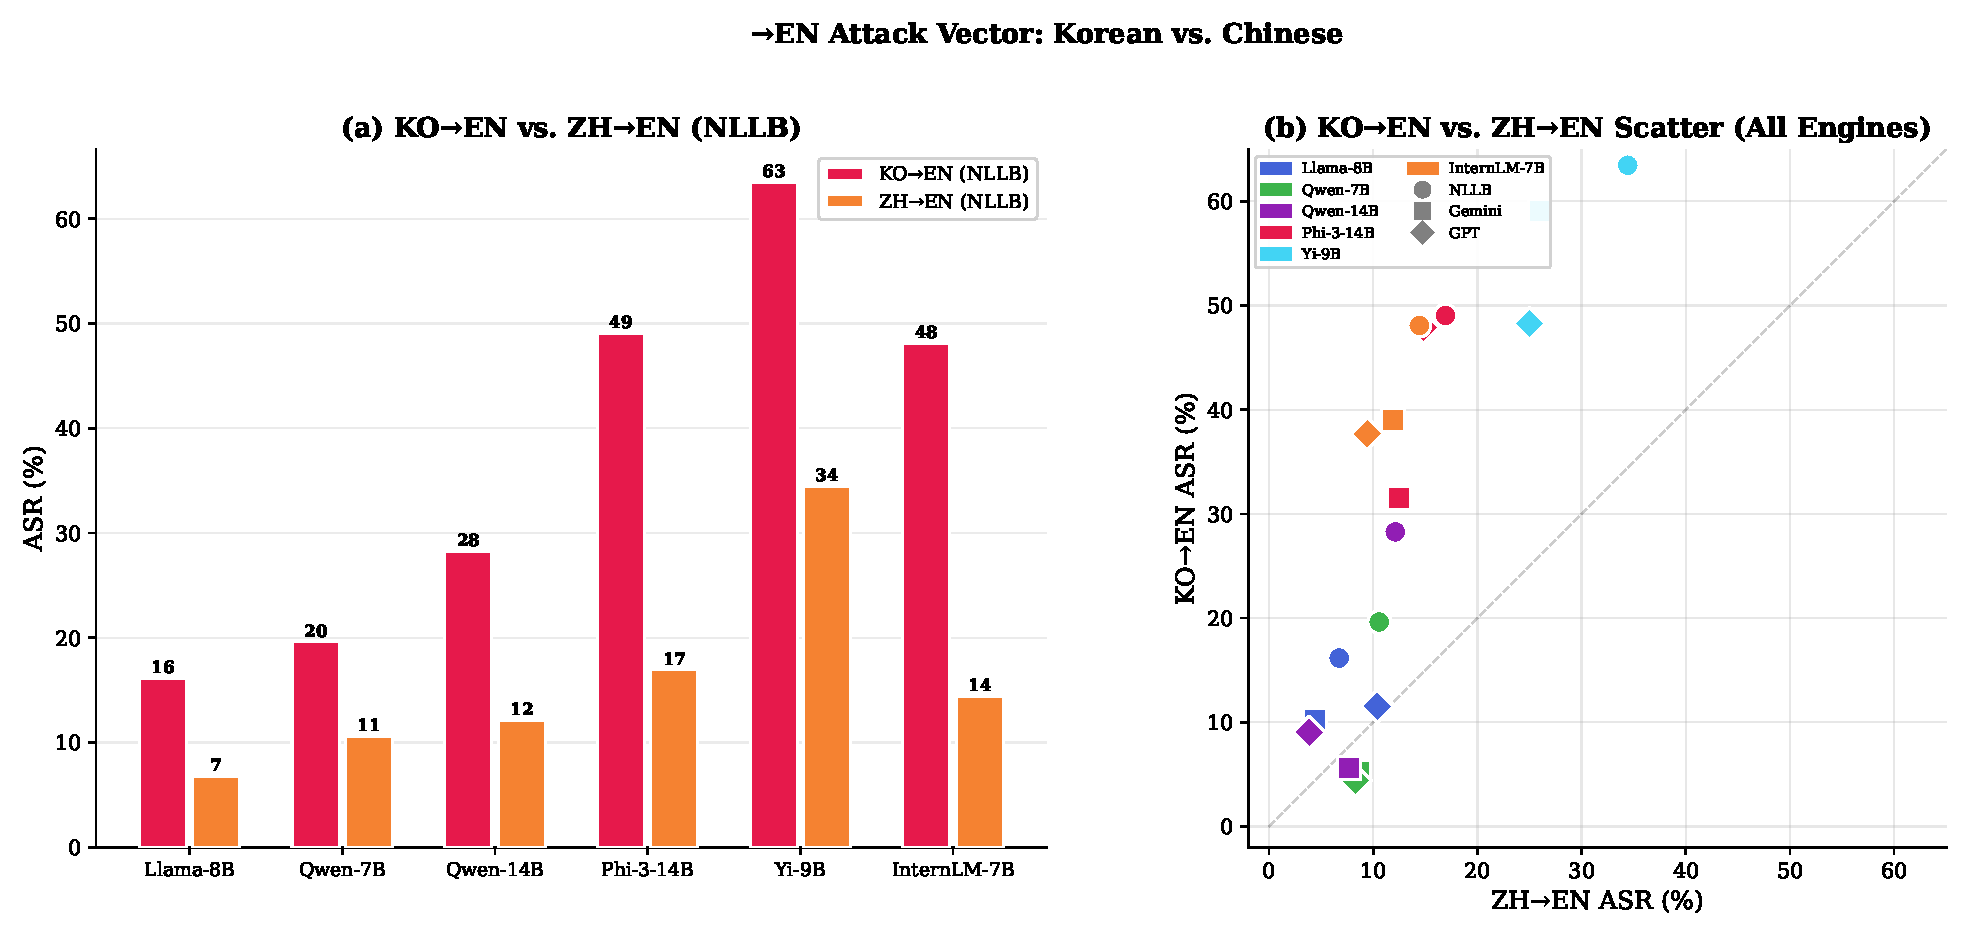
\includegraphics[width=\textwidth]{ko2en_analysis.pdf}
\caption{$\to$EN attack vector comparison.
(a)~KO$\to$EN (NLLB) vs.\ ZH$\to$EN (NLLB) by model.
(b)~Scatter of KO$\to$EN vs.\ ZH$\to$EN ASR across all
engines, showing KO$\to$EN is consistently more potent.}
\label{fig:x2en}
\end{figure*}

\subsection*{B. Content Language Dominance (MIX Conditions)}

Figure~\ref{fig:mix} confirms that preserving English content
within both Korean and Chinese instruction frames maintains
near-baseline safety, proving content-level detection.

\begin{figure*}[t]
\centering
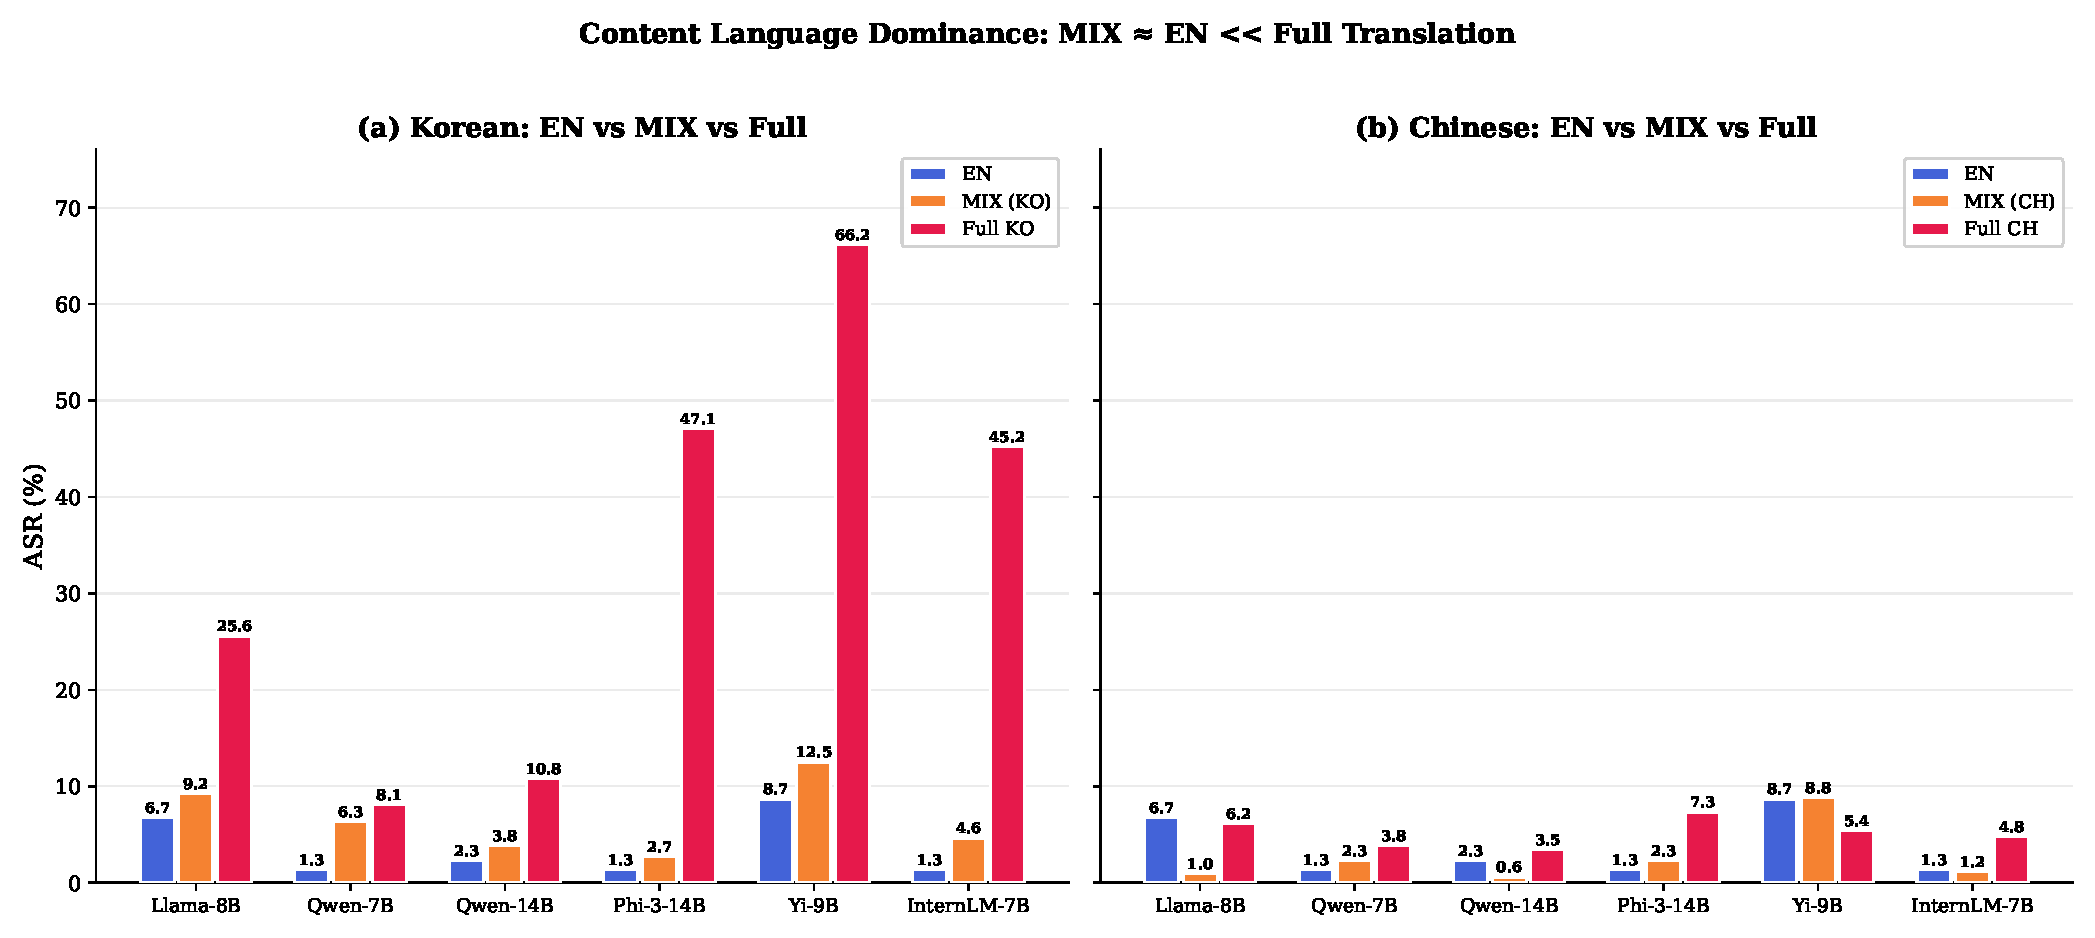
\includegraphics[width=\textwidth]{mix_vs_en.pdf}
\caption{Content language dominance: EN vs.\ MIX vs.\ full
translation for both Korean and Chinese.
MIX conditions closely track the EN baseline in both languages.}
\label{fig:mix}
\end{figure*}

\subsection*{C. Extended ASR Results}

Figure~\ref{fig:grouped_bar} presents the full grouped bar chart
across all seventeen conditions and six models.

\begin{figure*}[t]
\centering
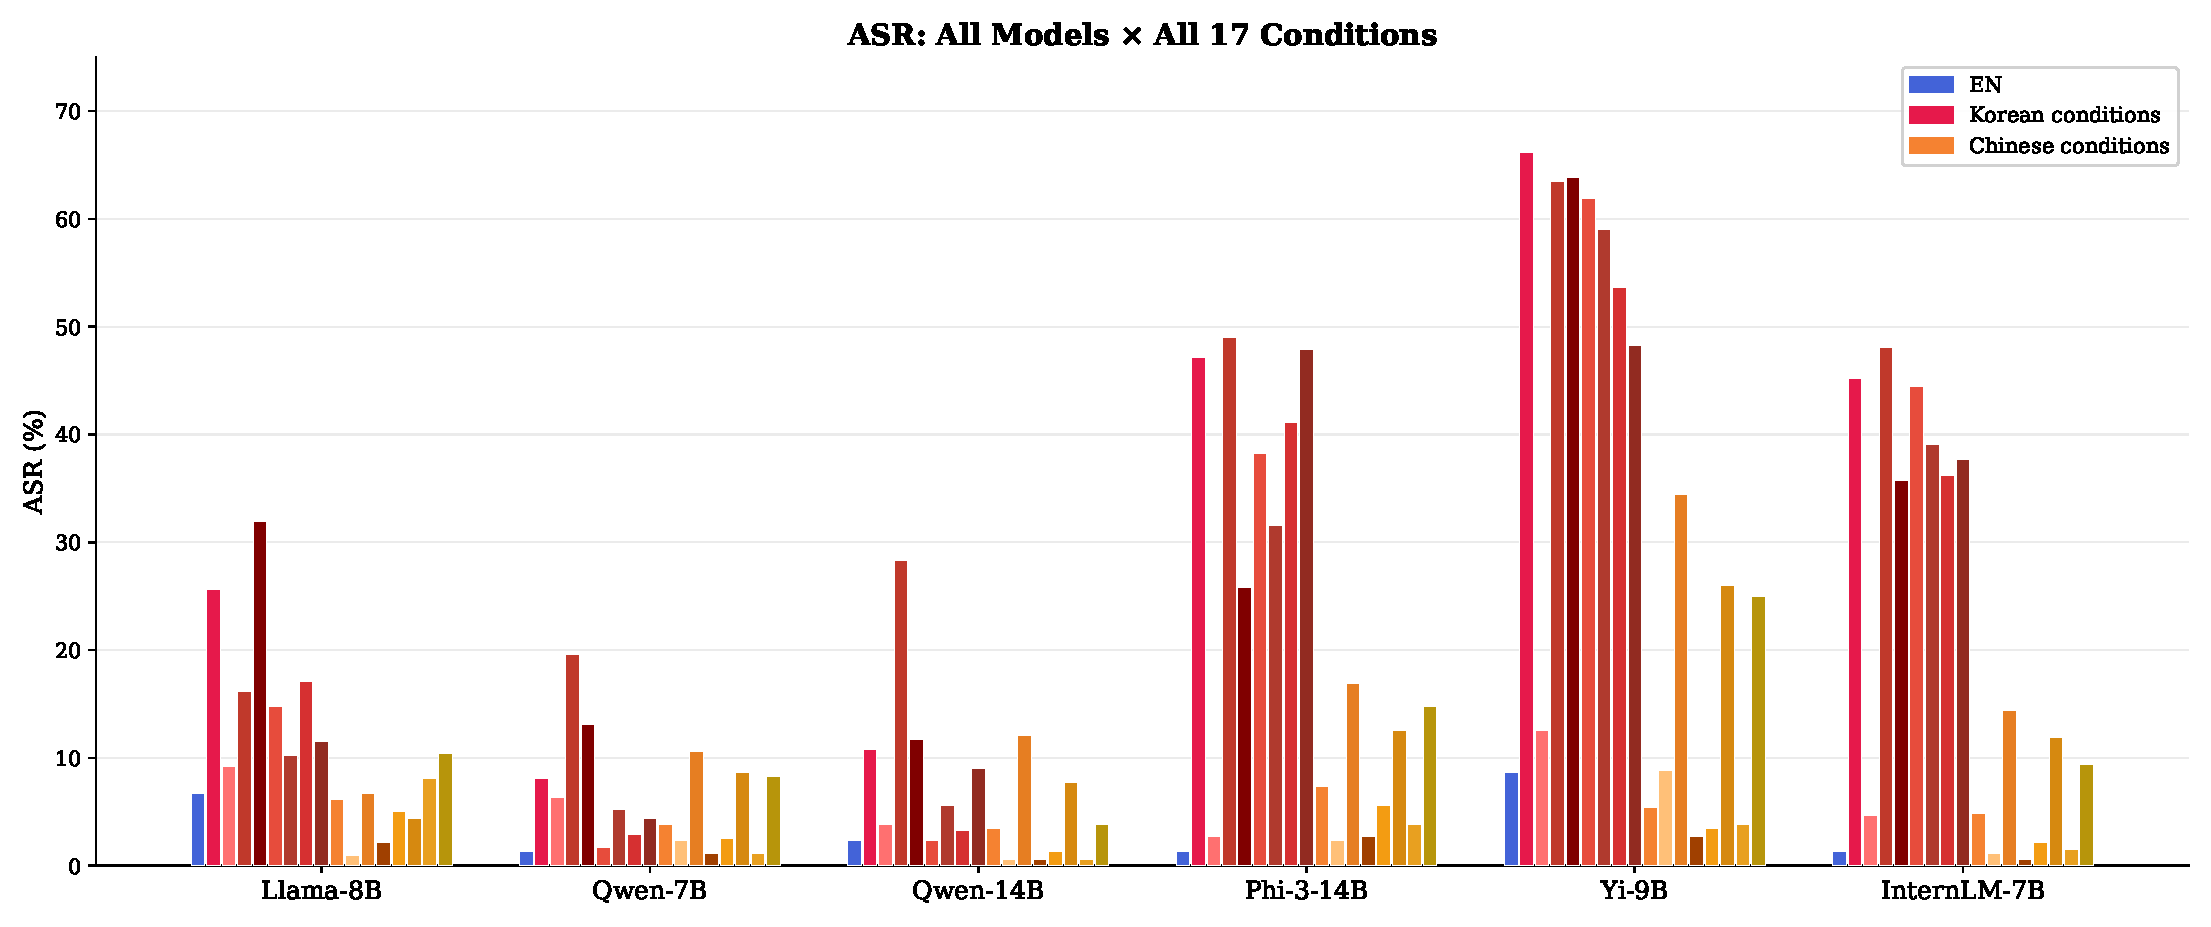
\includegraphics[width=\textwidth]{asr_grouped_bar_all.pdf}
\caption{Full grouped bar chart showing ASR for all 102
model--condition combinations.
Korean conditions (red shades) consistently produce higher ASR
than Chinese conditions (orange shades) across all models.}
\label{fig:grouped_bar}
\end{figure*}

\subsection*{D. Response Language Distribution}

Figure~\ref{fig:response_lang} shows response language distribution
per model across Korean conditions.

\begin{figure*}[t]
\centering
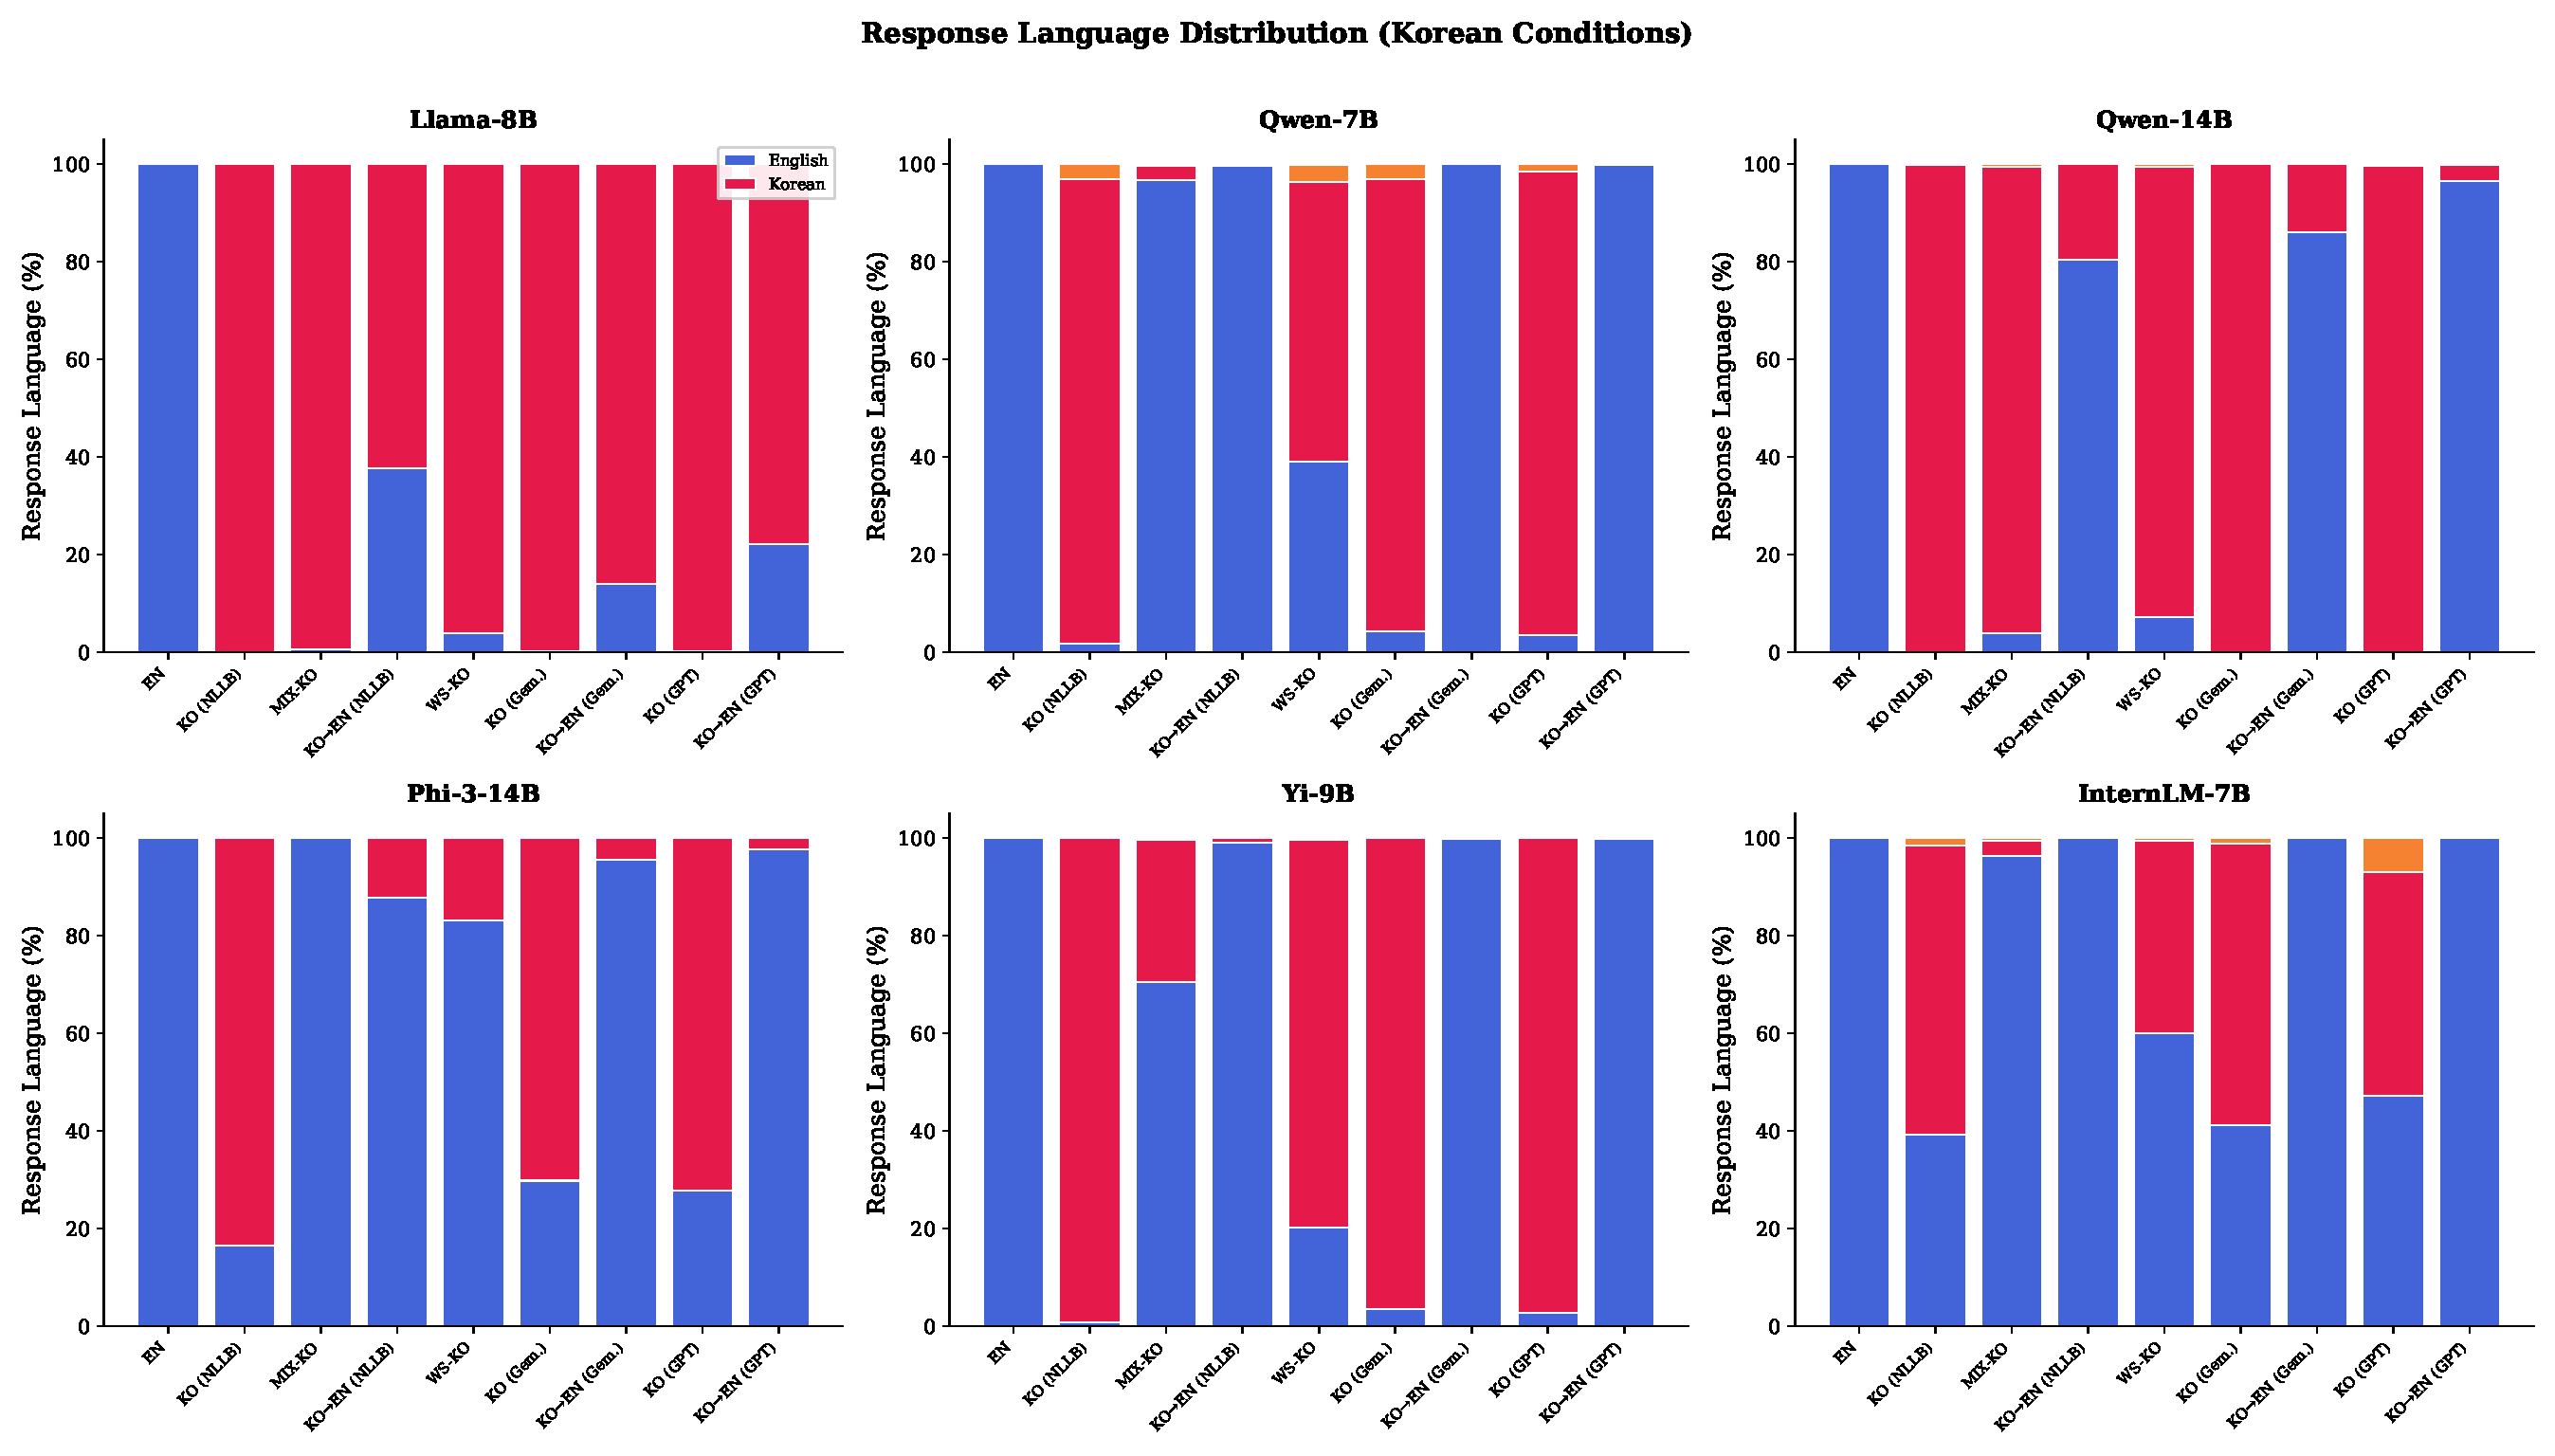
\includegraphics[width=\textwidth]{response_language.pdf}
\caption{Response language distribution by model for Korean conditions.}
\label{fig:response_lang}
\end{figure*}

\subsection*{E. Per-Model ASR Profiles (Radar Charts)}

Figure~\ref{fig:radar} presents bilingual radar charts showing each
model's ASR profile for Korean (red) and Chinese (orange) conditions.

\begin{figure*}[t]
\centering
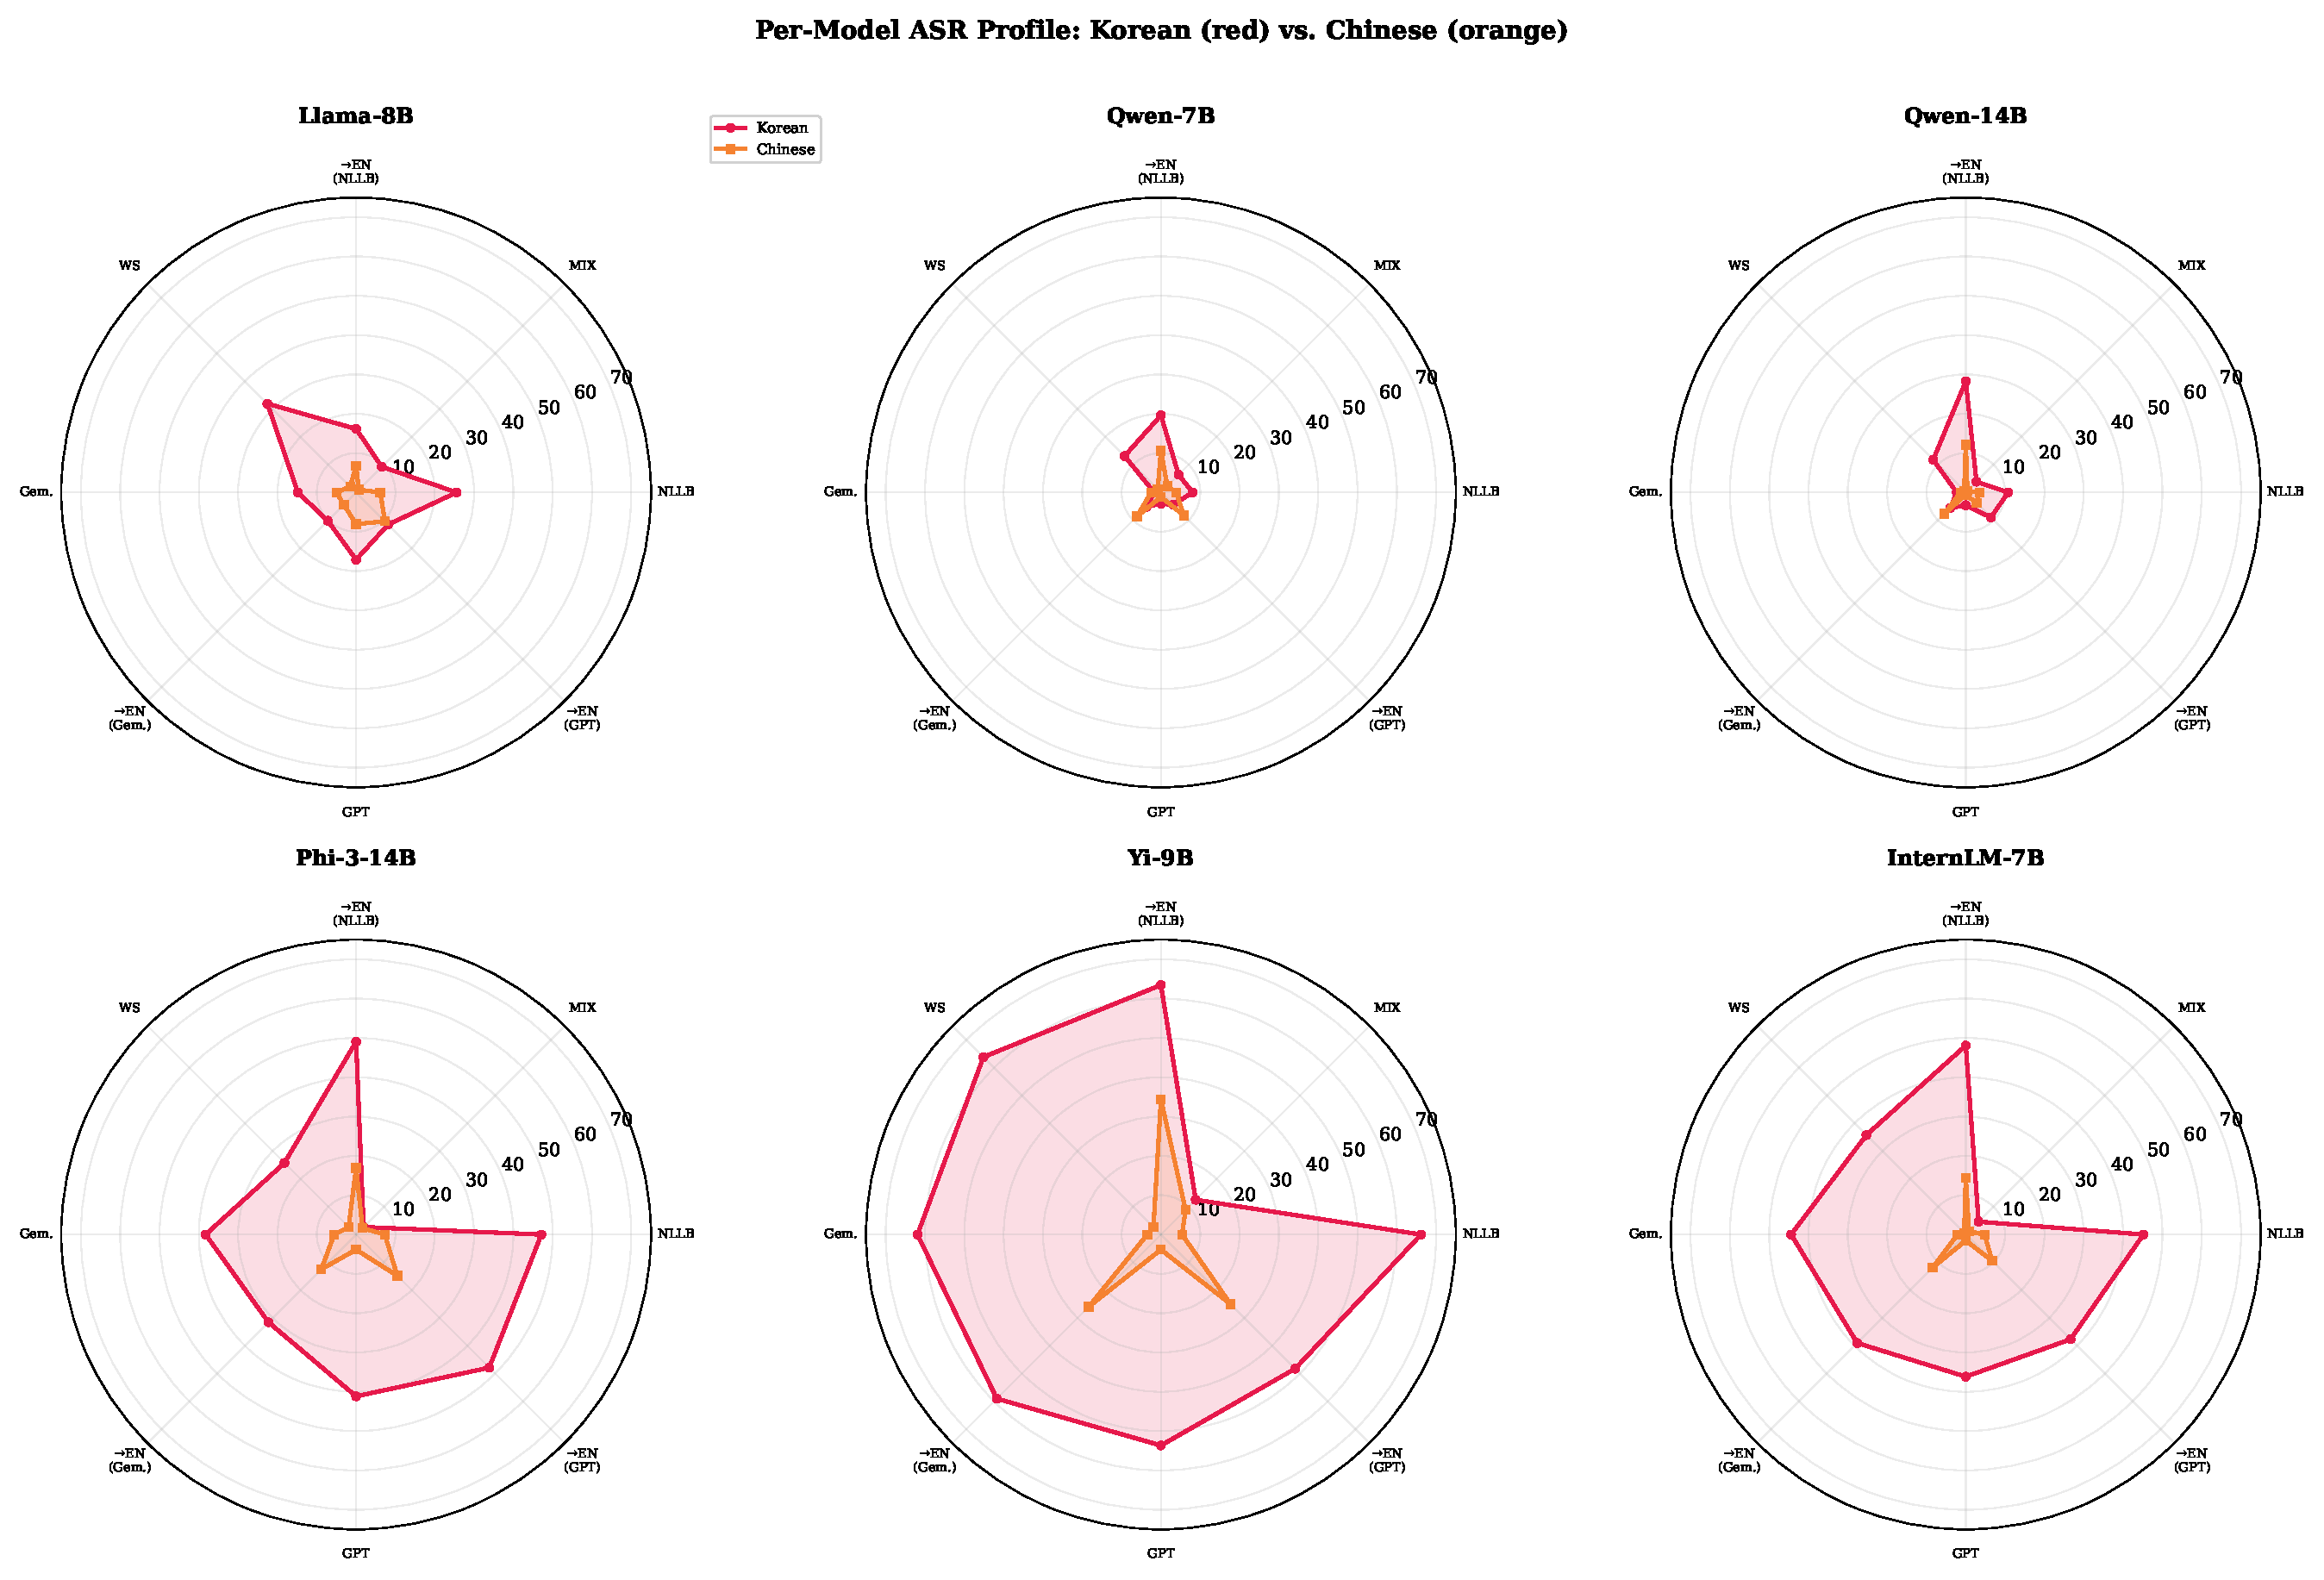
\includegraphics[width=\textwidth]{radar_per_model.pdf}
\caption{Per-model ASR profiles: Korean (red) vs.\ Chinese (orange).
Tier~2 models show inflated Korean profiles but flat Chinese profiles,
visualizing the language-specific safety gap.}
\label{fig:radar}
\end{figure*}

\subsection*{F. Category-Level ASR by Model}

Figure~\ref{fig:cat_detail} provides category-level ASR for each model.

\begin{figure*}[t]
\centering
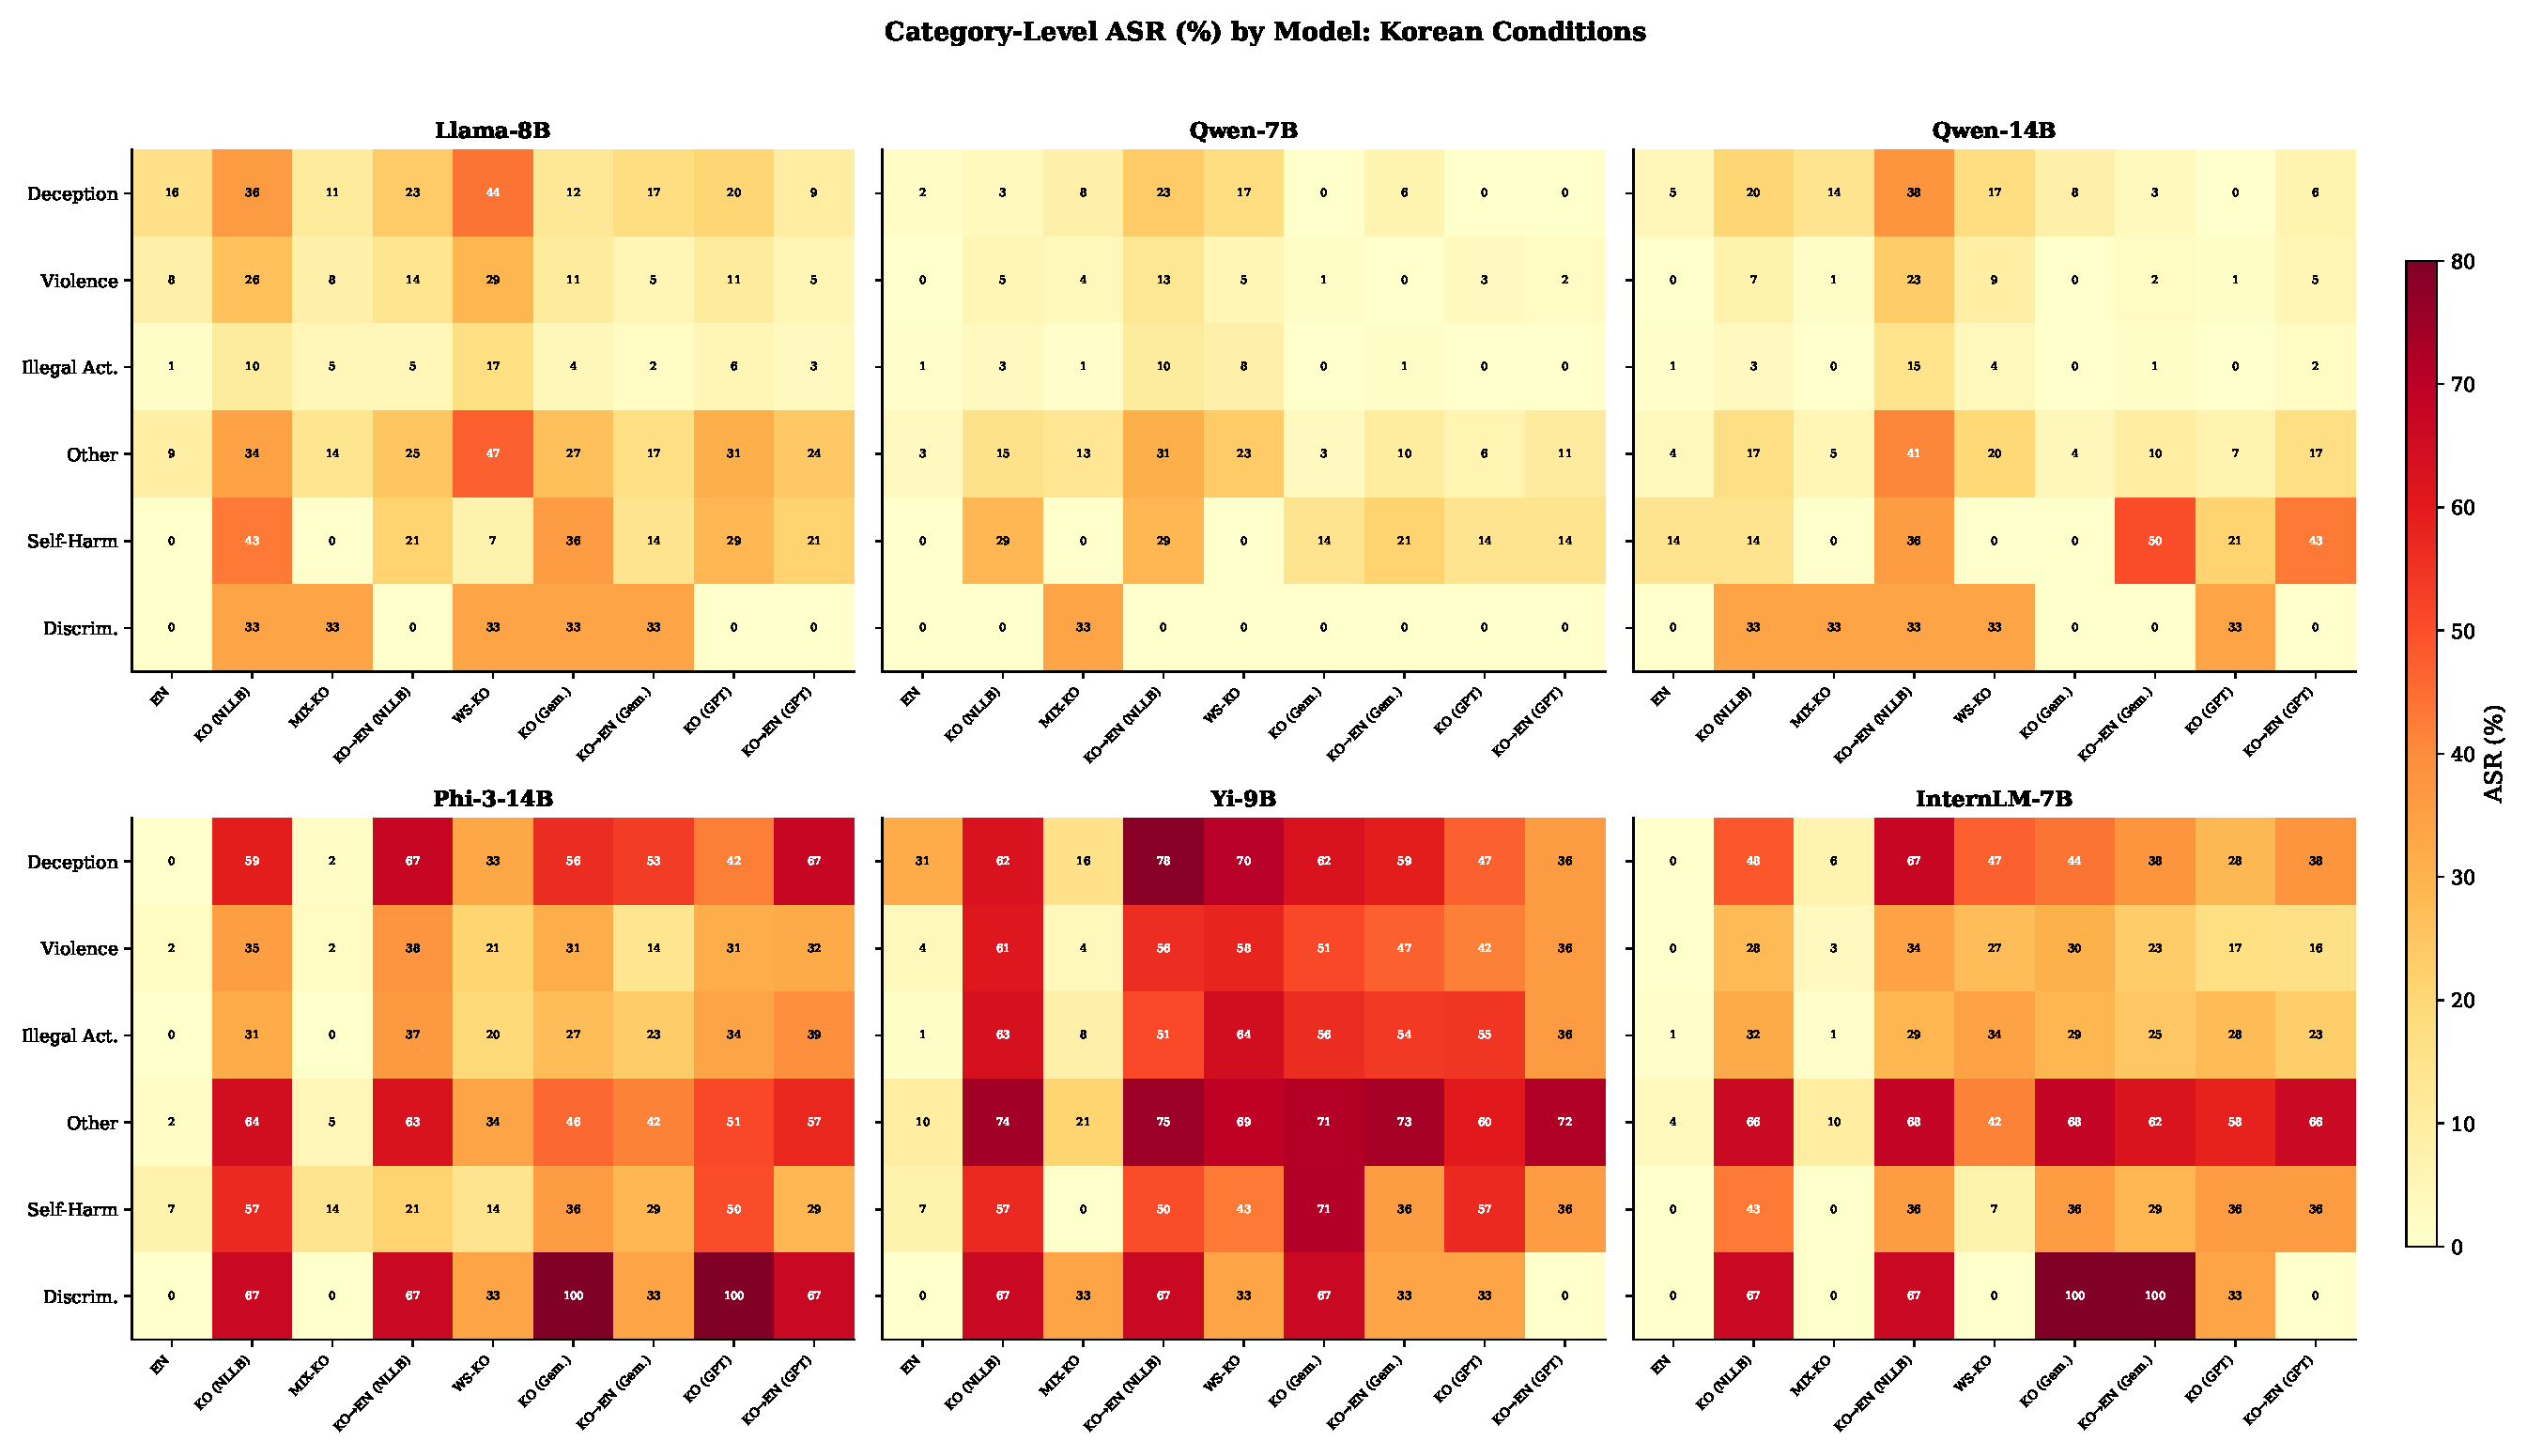
\includegraphics[width=\textwidth]{category_per_condition.pdf}
\caption{Category-level ASR (\%) by model across Korean conditions.}
\label{fig:cat_detail}
\end{figure*}

\subsection*{G. Language Capability vs.\ Safety}

Figure~\ref{fig:cap_safety} shows that language capability does not
predict safety degradation.

\begin{figure*}[t]
\centering
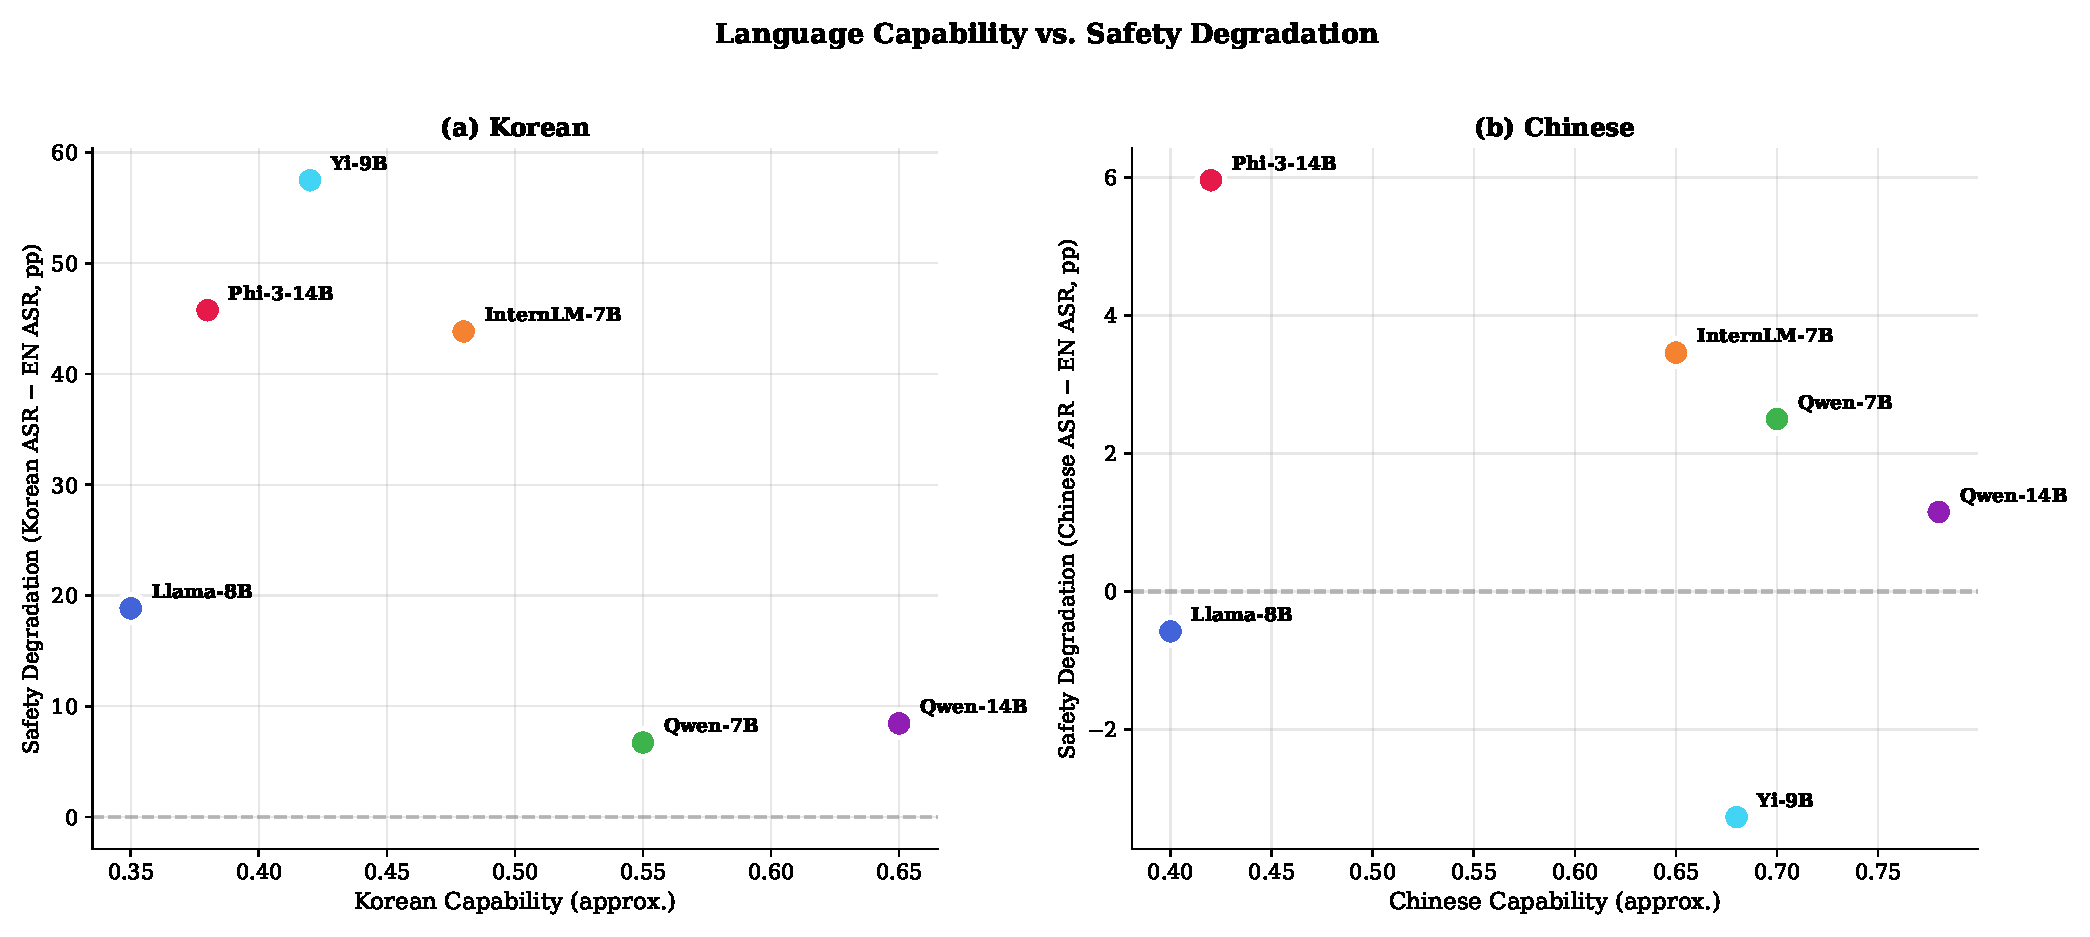
\includegraphics[width=\textwidth]{capability_vs_safety.pdf}
\caption{Language capability vs.\ safety degradation for
(a)~Korean and (b)~Chinese.
Korean shows no positive correlation.
Chinese shows minimal degradation regardless of capability.}
\label{fig:cap_safety}
\end{figure*}

\subsection*{H. Chinese Conditions Zoomed Heatmap}

Figure~\ref{fig:zoomed} provides a rescaled view of Chinese conditions.

\begin{figure*}[t]
\centering
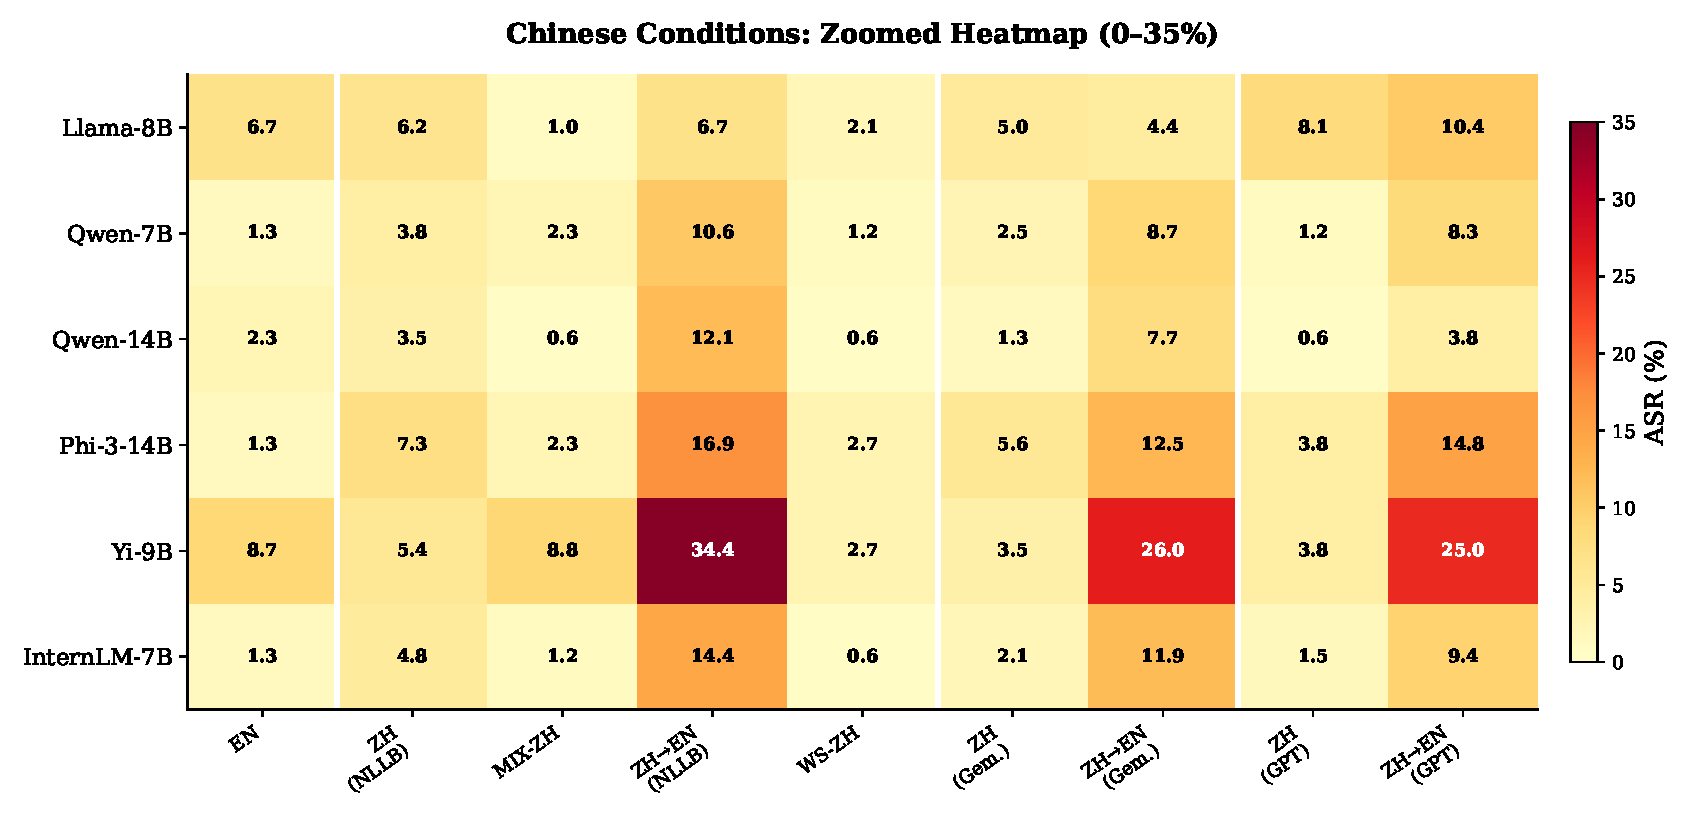
\includegraphics[width=\textwidth]{well_aligned_heatmap.pdf}
\caption{Chinese conditions heatmap (0--35\% scale) for fine-grained
comparison.
Even at this zoomed scale, most cells remain below 10\% ASR,
confirming strong Chinese safety across all models.
The ZH$\to$EN conditions show the only notable elevation.}
\label{fig:zoomed}
\end{figure*}

\subsection*{I. Amplification Factor by Language}

Figure~\ref{fig:amplification} compares the safety erosion
amplification factor across languages and engines.

\begin{figure*}[t]
\centering
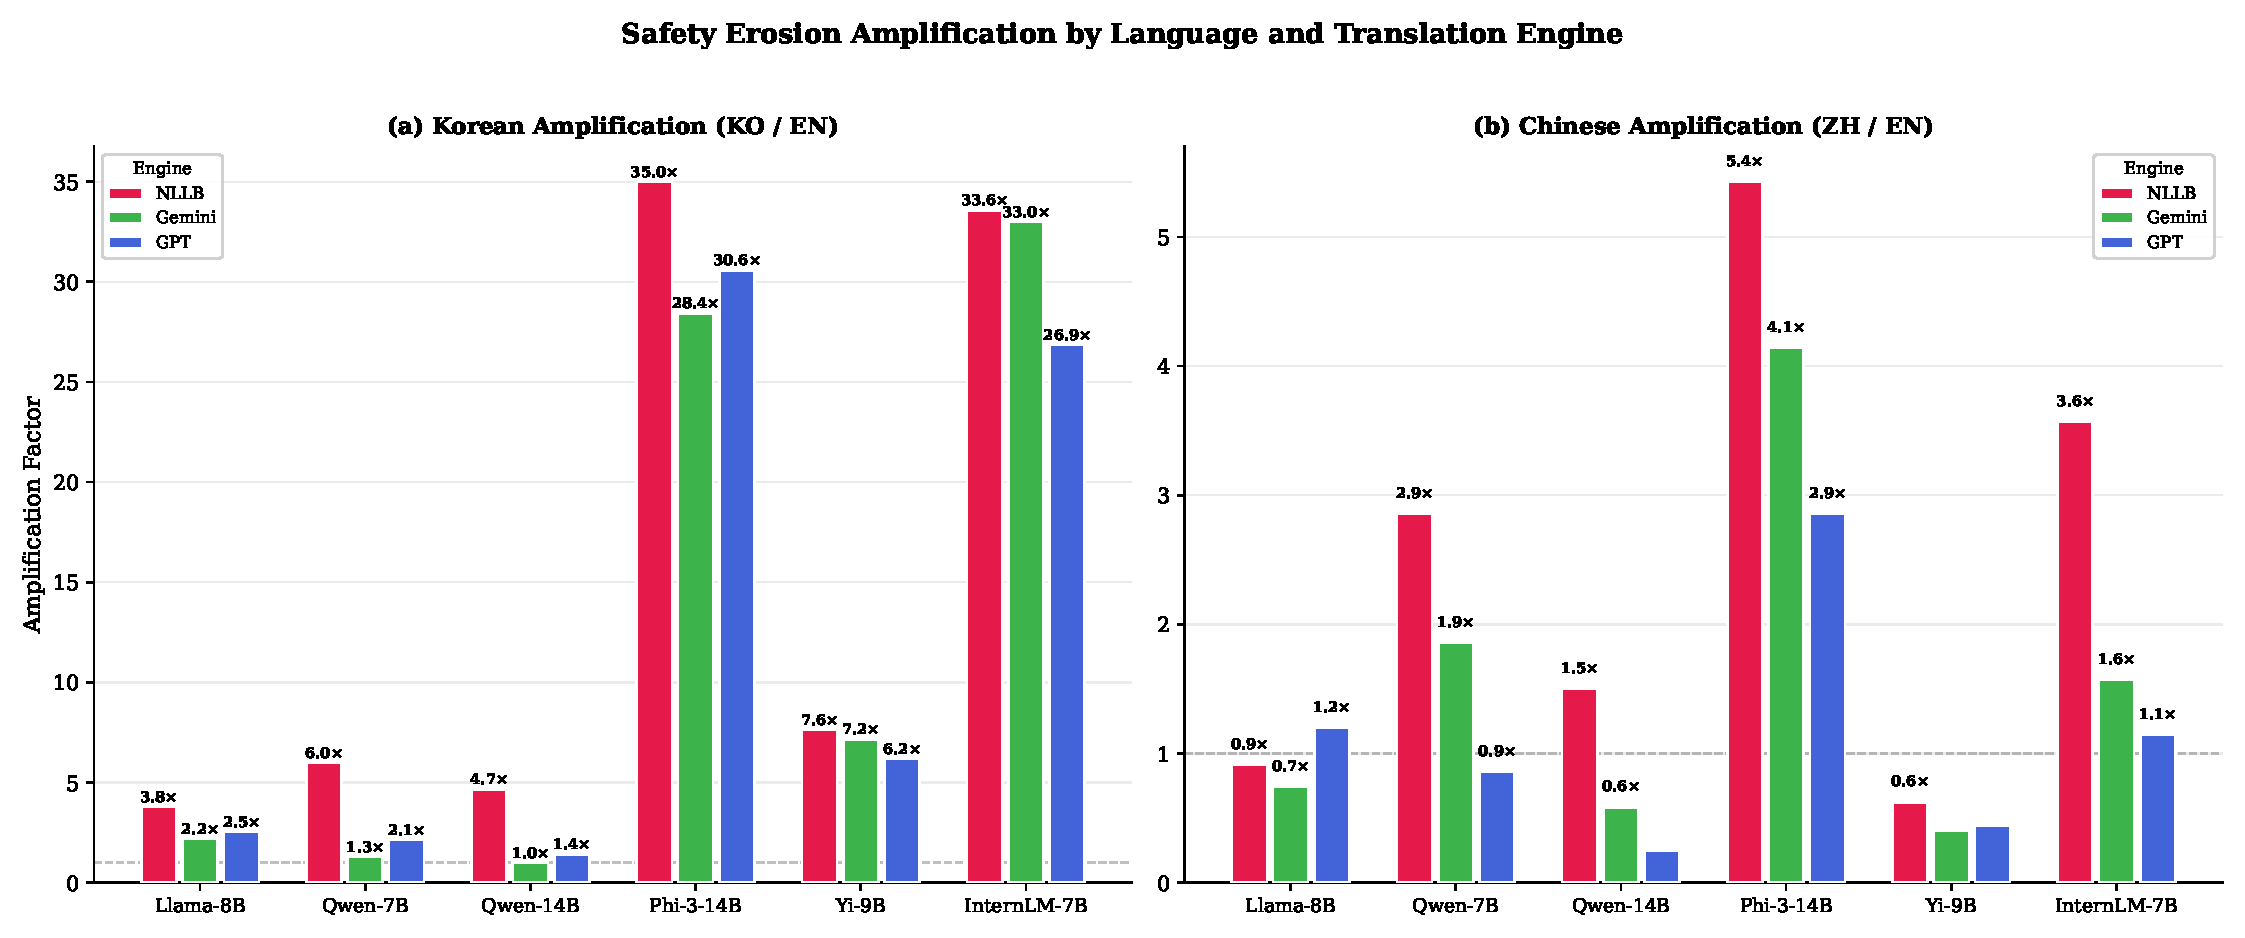
\includegraphics[width=\textwidth]{amplification_factor.pdf}
\caption{Safety erosion amplification factor
(target ASR / EN ASR) by language and engine.
(a)~Korean shows extreme amplification ($>$30$\times$ for
Phi-3 and InternLM with NLLB).
(b)~Chinese shows minimal amplification ($<$2$\times$ for most
model-engine combinations).}
\label{fig:amplification}
\end{figure*}

\end{document}
